\section{Méthode d'inventaire hors rue basée sur les codes d'urbanisme}\label{sec:meth_urb_based_inventory}
    %\subsection{Usages envisagés pour l'inventaire de stationnement}
    %Plusieurs usages sont envisagés pour la base de données de stationnement. Il est important de les expliciter puisque cela sera la base pour l'établissement de requis pour la structure des données. Les usages envisagés sont donc les suivants:
    %\begin{itemize}
   %     \item Étude d'accessibilité d'une place de stationnement à un lieu donnée (requiert que les places soient explicitées individuellement)
   %     \item Estimation du nombre de places de stationnement pour une destination précise
   %     \item Estimation du nombre de places de stationnement dans une zone d'analyse
    %    \item Analyse économétrique de l'effet de la tarification ou de la variation de l'offre sur les comportements de mobilité.
    %    \item Estimation de la surface minéralisée pour l'entreposage des voitures pour l'application d'écofiscalité   
    %\end{itemize}
    %Basé sur ces cas d'usage envisagés, la situation idéale serait d'avoir une base de données complètement désagrégée qui liste chaque place de stationnement. A minima, l'information doit être disponible au niveau du lot cadastral. D'autre part, il doit être possible d'encoder les informations relatives à la tarification de l'espace, le nombre disponible par lot , pour permettre d'appliquer des mesures d'écofiscalité. Il doit être possible d'agréger ces mesures au niveau à des zones d'analyse de déplacement pour faire des analyses sur la capacité de stationnement dans une zone dans un modèle de transport. \par
    %Ultimement, l'ensemble de ces requis soulève la nécessité d'une base de données personnalisée. En effet, dans le cas d'un inventaire basé sur la réglementation, \ac{OSM} est mal adapté puisqu'il requiert la localisation précise des places ce qui n'est pas nécessairement faisable. D'autre part, cela ne lie pas le stationnement à un identifiant qui permet à une entité gouvernementale d'appliquer cette fiscalité. Idéalement, la base de données serait capable d'exporter un format importable dans \ac{OSM} pour mettre à jour les données ouvertes au public.
    \subsection{Structure de la section}
        Cette section couvre de nombreux enjeux. La structure de cette section est la suivante: 
        \begin{itemize}
            \item Justification du niveau d'agrégation de l'inventaire
            \item Schéma relationnel de données pour ce mémoire
            \item Structure des données de l'inventaire final
            \item Structure des données de la géopolitique du territoire à l'étude
            \item Structure de données représentant les règlements
            \item Trois exemples de règlements
            \item Structure de données représentant l'ensemble des règlements applicables sur un territoire à une période donnée
            \item Structure des données cadastrales et de taxation foncière utilisées pour l'étude
            \item Structure des données représentant les secteurs d'analyse
            \item Objets informatiques utilisés dans le calcul de l'inventaire
            \item Logigramme de la procédure de calcul de l'inventaire
        \end{itemize}
    \subsection{Choix d'une unité d'inventaire}
    Idéalement, il serait possible d'avoir la localisation précise de chaque place de stationnement. Cela permettrait de déterminer l'accessibilité aux destinations de manière complètement désagrégée. Il est nécessaire que les places soient agrégées par lot cadastral pour que les municipalités puissent appliquer des mesures d'écofiscalité et distribuer les places de stationnement aux divers comptes de taxes sur un même lot. Finalement, l'utilisation du lot cadastral est pertinente puisque les requis sont souvent applicables à un lot qui, à sa construction, aura des usages bien définis. Le lot cadastral est donc choisi comme niveau d'agrégation principal pour cette méthode et est reflété dans la structure de données.
    \subsection{Schéma relationnel de données}
        La figure \ref{fig:offstreet_db_erd} montre la structure de la base de données utilisée pour l'estimation de l'offre de stationnement. De manière simplifiée, les \underline{règlements} sont réunis en \underline{ensembles de règlements}. Ces ensembles de règlements sont associés à un \underline{territoire}. Chaque territoire est associé à une \underline{période} où les limites géographiques des municipalités sont restées stables.
        \begin{landscape}
        \begin{figure}
            \centering
            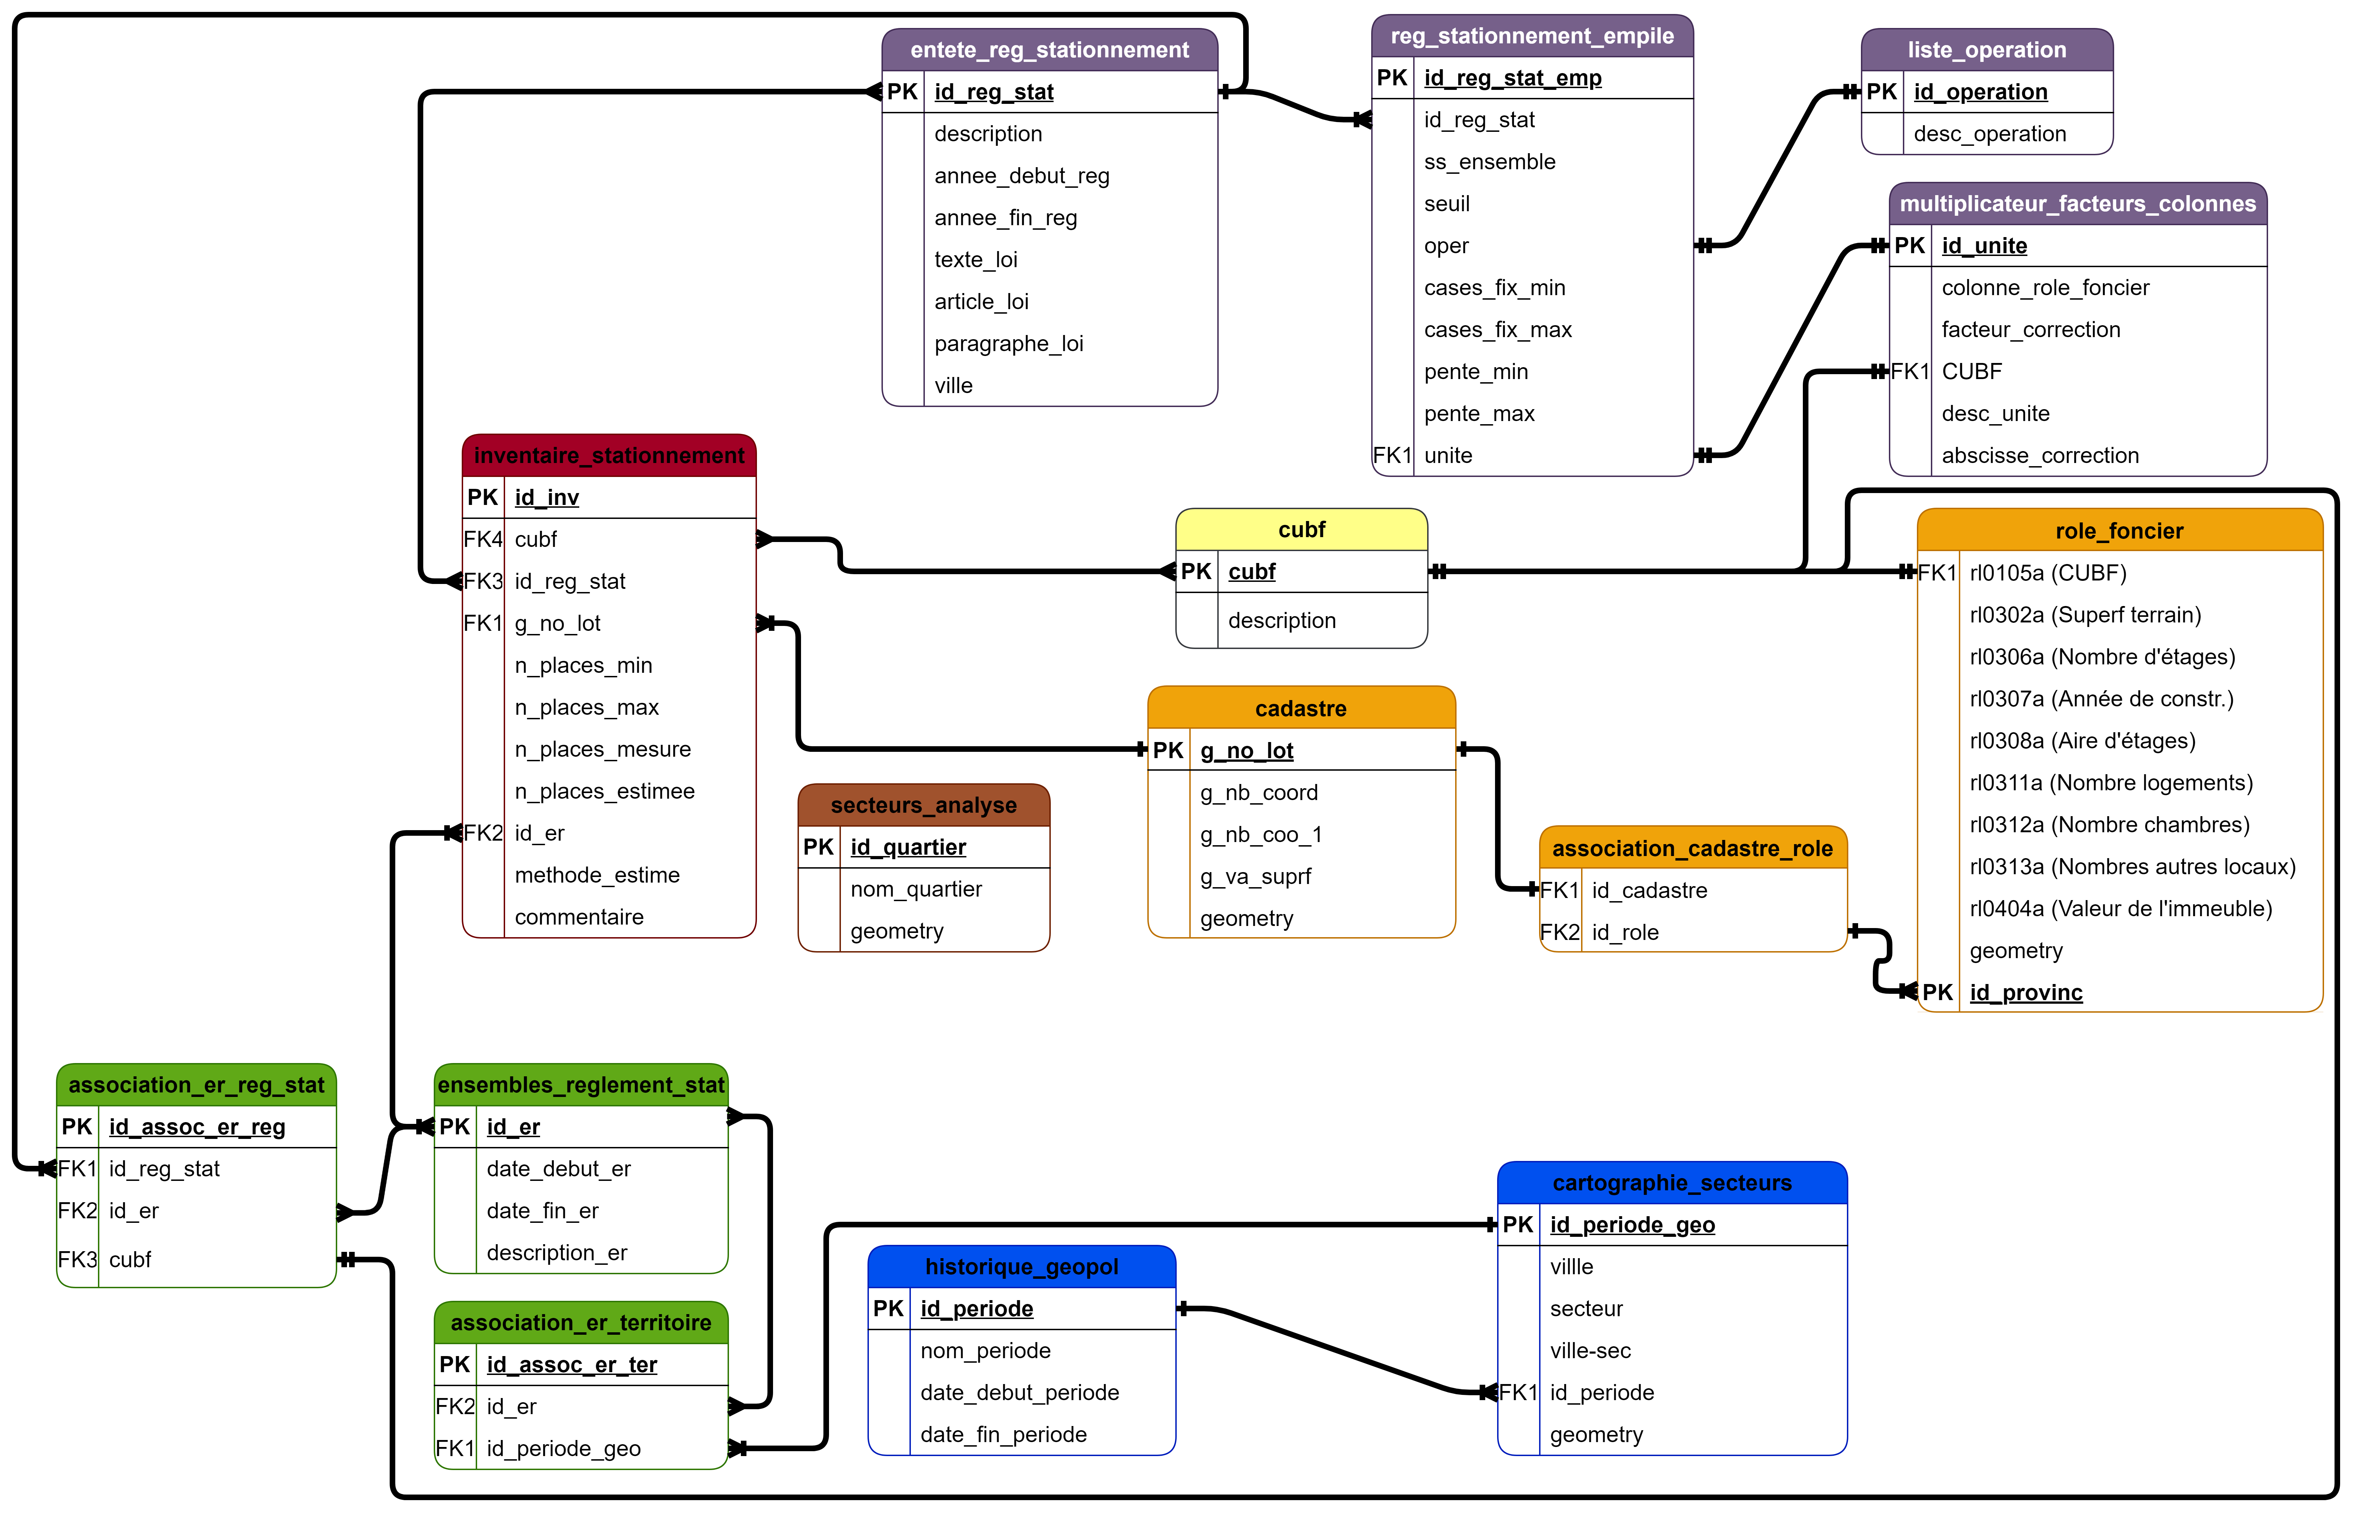
\includegraphics[width = 0.85\linewidth]{dia/ERD_stationnement_propre.png}
            \caption{Diagramme entité association de la base de données}\label{fig:offstreet_db_erd}
        \end{figure}
        \end{landscape}
        La base de données est implémentée dans PostgreSQL avec PostGIS pour pouvoir gérer les données spatiales du rôle foncier, du cadastre ainsi que de la division géopolitique du territoire.\par
    \subsection{Structure des données de l'inventaire final}
    La table \underline{inventaire\_stationnement} contient l'inventaire de stationnement. La table laisse la possibilité d'avoir plusieurs estimations par lot cadastral. Ainsi, l'usager peut utiliser une estimation réglementaire, entrer une valeur manuellement ou utiliser une méthode d'estimation basée sur les orthophotos pour remplir cette table. La table \ref{tab:definition_table_inventaire} résume les champs, le type de données et les en-têtes de la table:
    \begin{table}[h]
        \centering
        \begin{tabular}{m{0.2\textwidth}|m{0.4\textwidth}m{0.15\textwidth}m{0.075\textwidth}}
            \hline
            Nom champ & Description & Type de données & CP/CS  \\
            \hline
            id\_inv & Clé primaire  & Serial & CP \\ 
            n\_places\_min & Nombres de places minimales requises par la code d'urbanisme & Nombre réel &\\ 
            n\_places\_max & Nombres de places minimales requises par la code d'urbanisme & Nombre réel & \\ 
            n\_places\_estime & Nombres de places estimées si une méthode automatique est utilisée & Nombre réel&\\ 
            n\_places\_mesure & Entrée manuelle du nombres de places de stationnement & Nombre réel&\\
            methode\_estime & Champ pour indiquer le type d'estimé pour la ligne & \makecell[l]{Entier\\
                                                                                             1 - Manuel\\
                                                                                             2 - Régl.\\
                                                                                             3 - Orthophoto\\
                                                                                             4 - Autre}  & \\ 
            id\_reg\_stat & Règlements utilisés pour générer l'estimé. Si plusieurs sont utilisés, il peuvent être séparés par des virgules ou \textbackslash & Texte & \\ 
            id\_er & Ensembles de règlements utilisés pour générer l'estimé. Si plusieurs sont utilisés, il peuvent être séparés par des , ou des \textbackslash & Texte & \\ 
            commentaire & Texte contenant un commentaire au besoin & Texte & \\ 
            g\_no\_lot & Identifiant du lot pour l'inventaire & Texte & \\
            \hline
       \end{tabular}
       \caption{Colonnes pour la table \underline{inventaire\_stationnement}}
       \label{tab:definition_table_inventaire}
   \end{table}\par
    %La table \underline{entete\_tarifs} est la table contenant une description et une clé primaire d'identifiant de tarifs vers laquelle pointe la table d’inventaire. La table \underline{association\_tarifs} joint une période tarifaire, un tarif et l'identifiant de tarif. La table \underline{periode\_tarifaire} permet de définir des périodes de validité. Chaque période tarifaire a un identifiant unique, un identifiant de jours, une heure de début et une heure de fin. \par
    %Les tarifs ont chacun un entête avec un identifiant et une description entreposés dans la table \underline{entete\_couts\_tarifs}. La table \underline{couts\_tarifaires} contient les données de tarification. La structure a été ainsi faite pour permettre plusieurs types de tarification en fonction de l'heure de la journée et une progression de la tarification. Les champs de la table sont type\_couts qui définit s'il s'agit d'un abonnement un paiement à l'entrée ou un paiement en sortie. Le champ seuil\_temps et unite\_seuil définissent un seuil au-delà duquel le tarif s'applique. Les champs ordonnee\_origine, pente\_tarif, unite\_tarif définissent l'ordonnée à l'origine, la pente et l'unité à fournir entrée pour obtenir le prix du stationnement.\par
    %Pour conclure, la table \underline{clienteles\_hors\_rue} définit l'association entre le type de clientèle et l'entier enregistré dans la table \underline{inventaire\_stationnement}. Les valeurs possibles envisagées sont listées au tableau \ref{tab:clienteles_hors_rue}.
    %\begin{table}
    %\centering
    %\begin{tabular}{l l}
    %\hline
    %id\_clientèle & Description clientèle\\ \hline
    %0& Automobiles - Propriétaire et Visiteurs Autorisés \\
    %1 & Automobiles - Propriétaires Seulement \\
    %2 & Automobiles - Clients \\
    %3 & Automobiles - Employés seulement \\
    %4 & Automobiles - Véhicules autorisés \\
    %5 & Automobiles - Vignettes résidents \\
    %6 & Automobiles - Vignettes Autres \\
    %7 & Automobiles - Tous\\ \hline
    %\end{tabular}
    %\caption{Entrées dans la table \underline{clienteles\_hors\_rue}}\label{tab:clienteles_hors_rue}
    %\end{table}
    \FloatBarrier
    %La figure \ref{fig:offstreet_db_erd_output} montre le détail de la base de données discutée dans cette section. Cette structure permet de séparer les places disponibles aux différentes clientèles de manière extensible pour chaque lot et de répertorier des structures de tarification complexes au besoin.
    %\begin{figure}[!h]
    %    \centering
    %    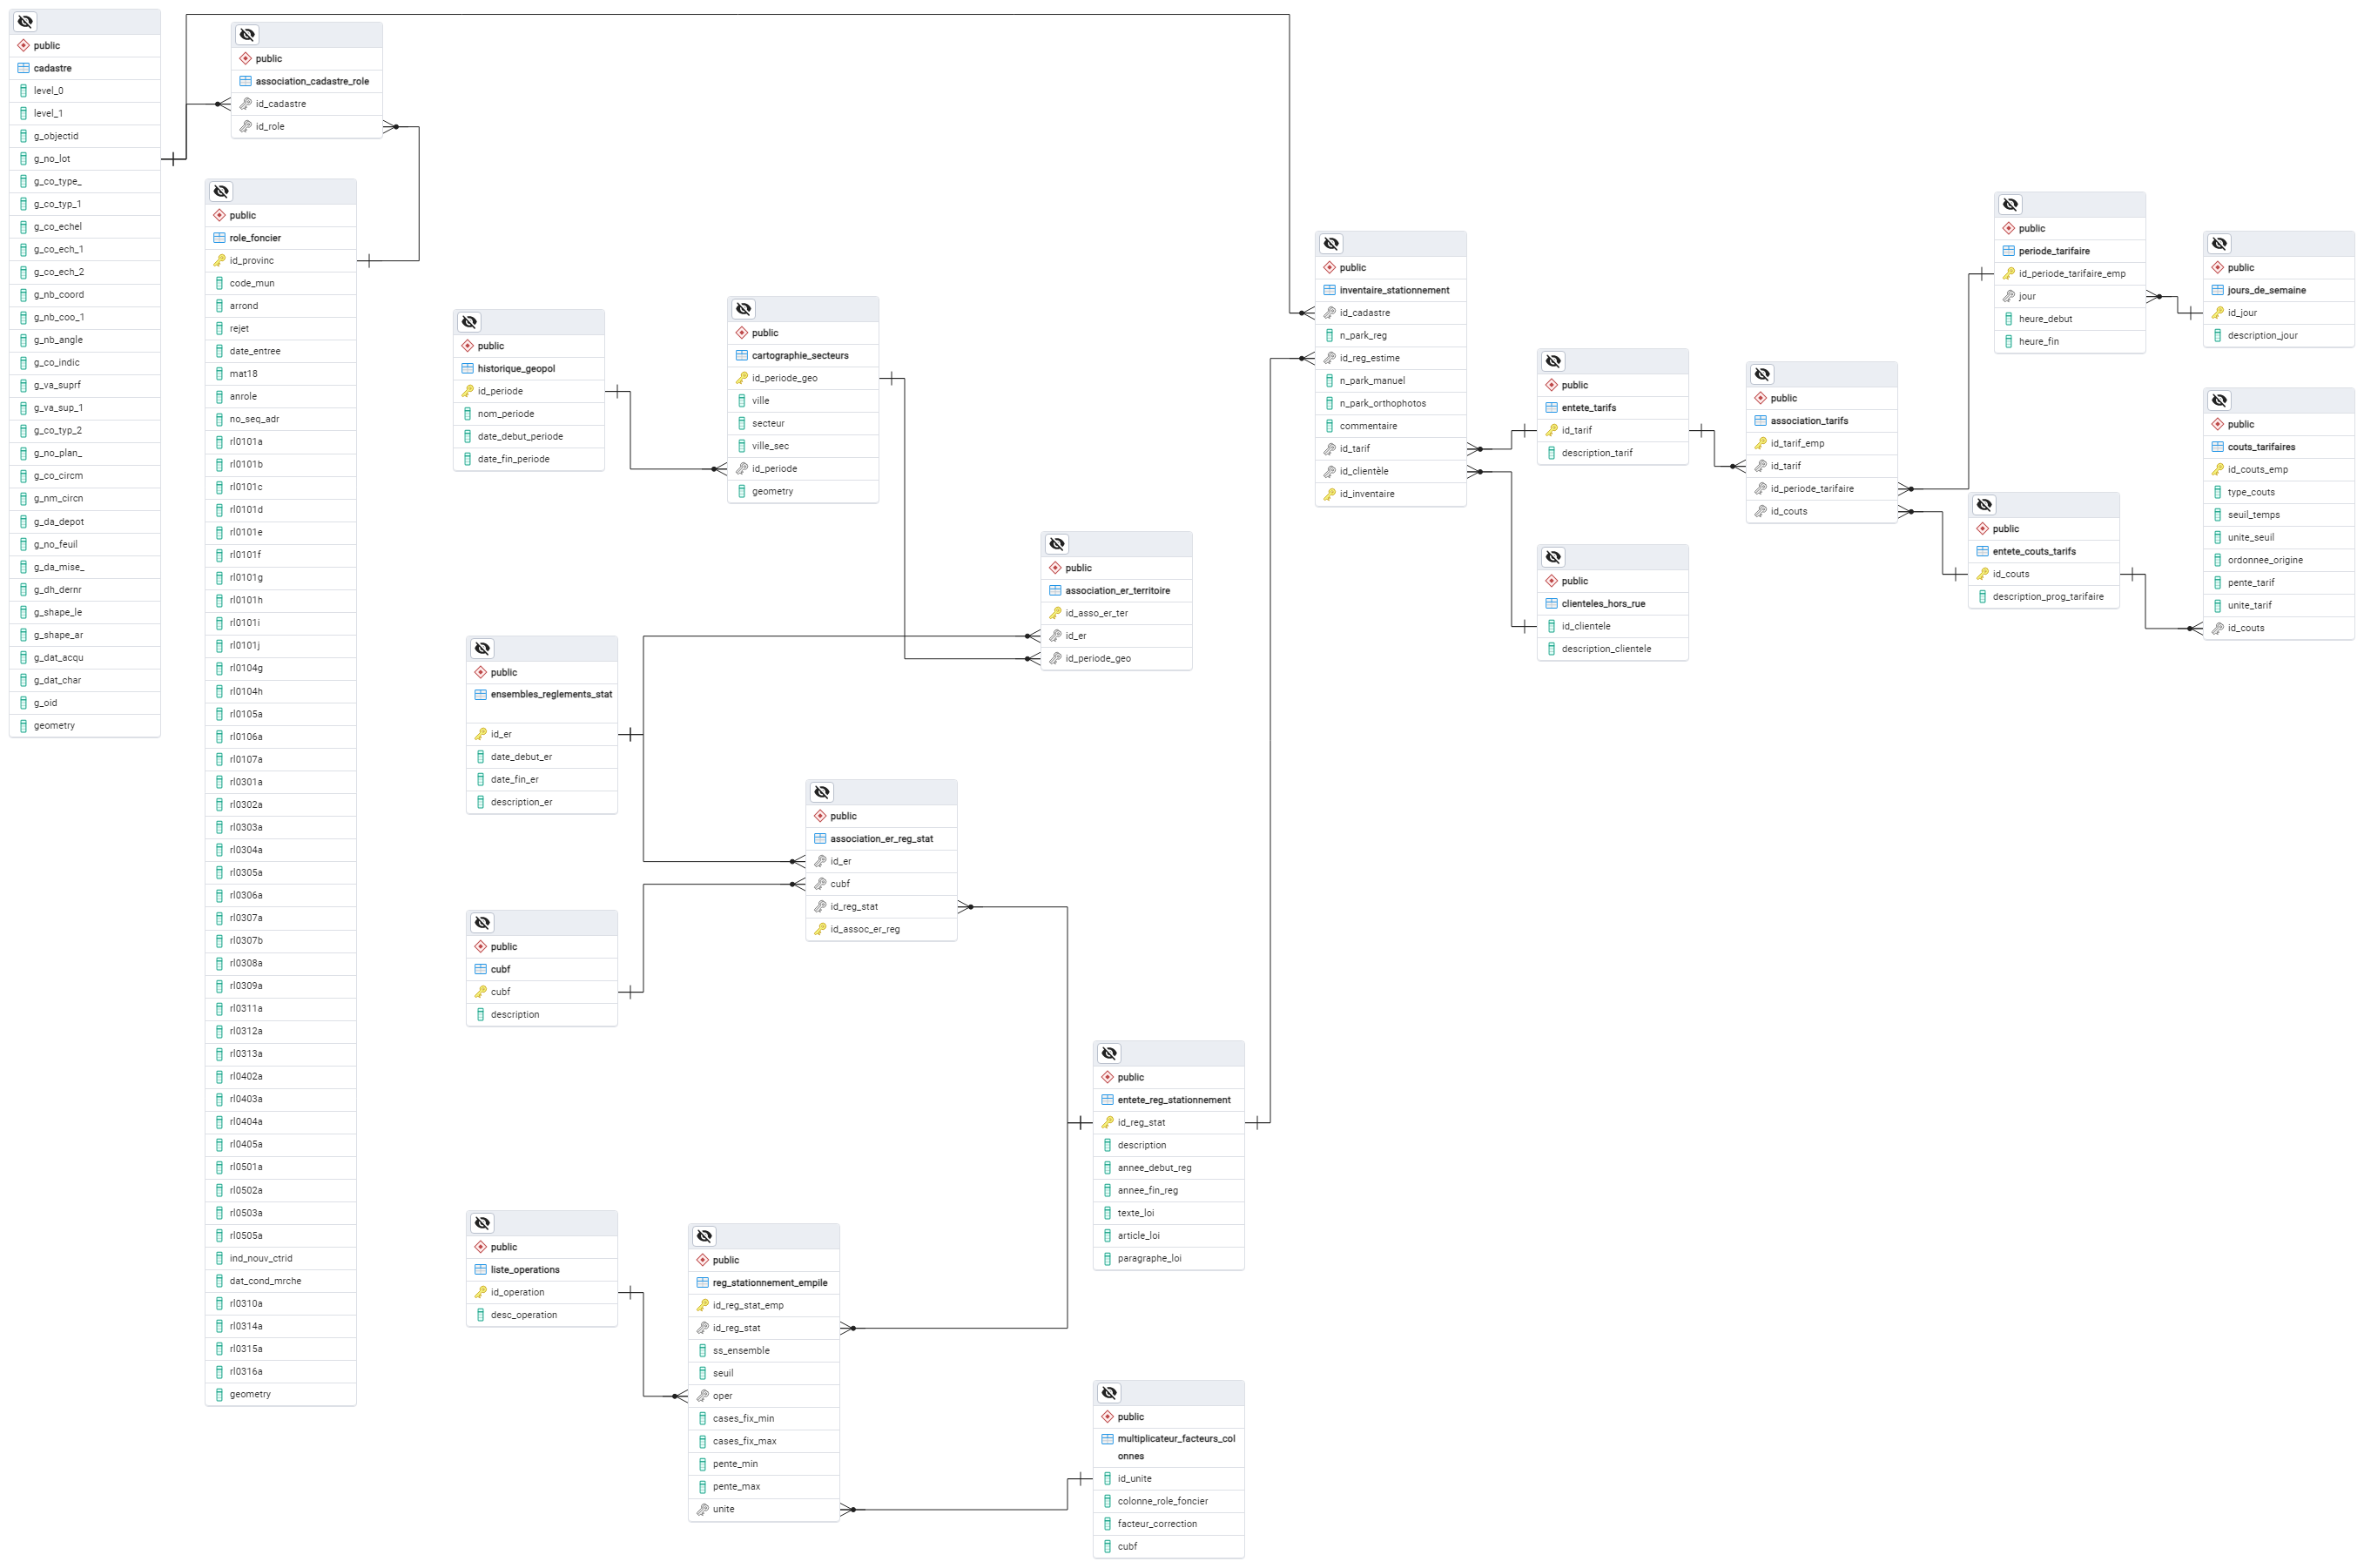
\includegraphics[trim={50cm 35cm 0 7cm}, clip, width=14cm]{images/structure_base_de_donnee.png}
    %    \caption{Structure de données en sortie de procédure de calcul}\label{fig:offstreet_db_erd_output}
    %\end{figure}
    %\FloatBarrier

    
    \subsection{Structure des données de la géopolitique du territoire à l'étude} 
    Les règlements régissant la capacité de stationnement changent dans le temps aux aléas des élus et des variations spatiales des municipalités. Il est donc nécessaire de représenter l'historique géopolitique de la métropole. Cet historique est représenté au moyen de deux tables: \underline{historique\_geopol} et \underline{cartographie\_secteurs}. \underline{historique\_geopol} représente les grandes périodes où le territoire a été stable. 
    Le tableau \ref{tab:definition_historique_geopol} montre les colonnes de la table {historique\_geopol} \par
    \begin{table}[h]
       \centering
       \begin{tabular}{m{0.25\textwidth}|m{0.3\textwidth}m{0.15\textwidth}m{0.075\textwidth}}
            \hline
            Nom champ & Description & Type de données & CP/CS  \\
            \hline
            id\_periode & Clé primaire  & Serial & CP \\ 
            nom\_periode & Nom de la période à montrer & Texte & \\ 
            date\_debut\_periode & Année de début de la période & Entier & \\ 
            date\_fin\_periode & Année de fin de la période& Entier & \\ 
            \hline
       \end{tabular}
       \caption{Colonnes pour la table \underline{historique\_geopol}}
       \label{tab:definition_historique_geopol}
   \end{table}\FloatBarrier
   Le tableau \ref{tab:definition_cartographie_secteurs} montre les colonnes de la table \underline{cartographie\_secteurs}. Cette table sépare le territoire d'étude en municipalités pour la période définie dans la colonne id\_periode.\par
    \begin{table}[h]
       \centering
       \begin{tabular}{m{0.2\textwidth}|m{0.4\textwidth}m{0.15\textwidth}m{0.075\textwidth}}
            \hline
            Nom champ & Description & Type de données & CP/CS  \\
            \hline
            id\_periode\_geo & Clé primaire  & Serial & CP \\ 
            id\_periode & Colonne d'association à l'historique & Entier & CS\\ 
            ville & Nom de la ville & Texte & \\ 
            secteur & Secteur de la ville & Texte & \\ 
            geometry & Géométrie du secteur & Géométrie & \\
            \hline
       \end{tabular}
       \caption{Colonnes pour la table \underline{cartographie\_secteurs}}
       \label{tab:definition_cartographie_secteurs}
    \end{table}
    \FloatBarrier \clearpage
    Dans le cas de la ville de Québec, 6 grandes périodes ont été identifiées \parencite{ville_de_quebec_reperes_nodate,elections_quebec_atlas_2021}. Elles sont listées au tableau \ref{tab:histo_geopol}.\par
    \begin{table}[h]
    \centering
    \begin{tabular}{c p{5cm} c c}
    \hline
    \makecell{Identifiant\\ id\_periode} & \makecell[l]{Nom \\ nom\_periode} & \makecell{Année début \\ date\_debut\_periode} & \makecell{Année fin \\ date\_fin\_periode}\\ \hline
    1 & Fondation - 1970 &  S.V. & 1970 \\
    3 & Duberger, Saules et Neufchâtel fusion Québec & 1971 & 1975 \\
    4 & Fusions Charlesbourg & 1976 & 1994 \\
    5 & Inauguration VQZ-3 & 1995 & 1996 \\
    6 & Abrogation Zone Prioritaire Ville de Québec & 1997 & 2009 \\
    7 & Harmonisation & 2010 & S.V.\\ \hline
    \end{tabular}
    \caption{Valeurs dans l'historique géopolitique utilisé dans le cadre de ce mémoire}\label{tab:histo_geopol}
    \end{table}
    La figure \ref{fig:offstreet_db_erd_history} montre le détail de la section de base de données montrant l'évolution des variations géopolitiques du territoire.
    \begin{figure}[h]
        \centering
        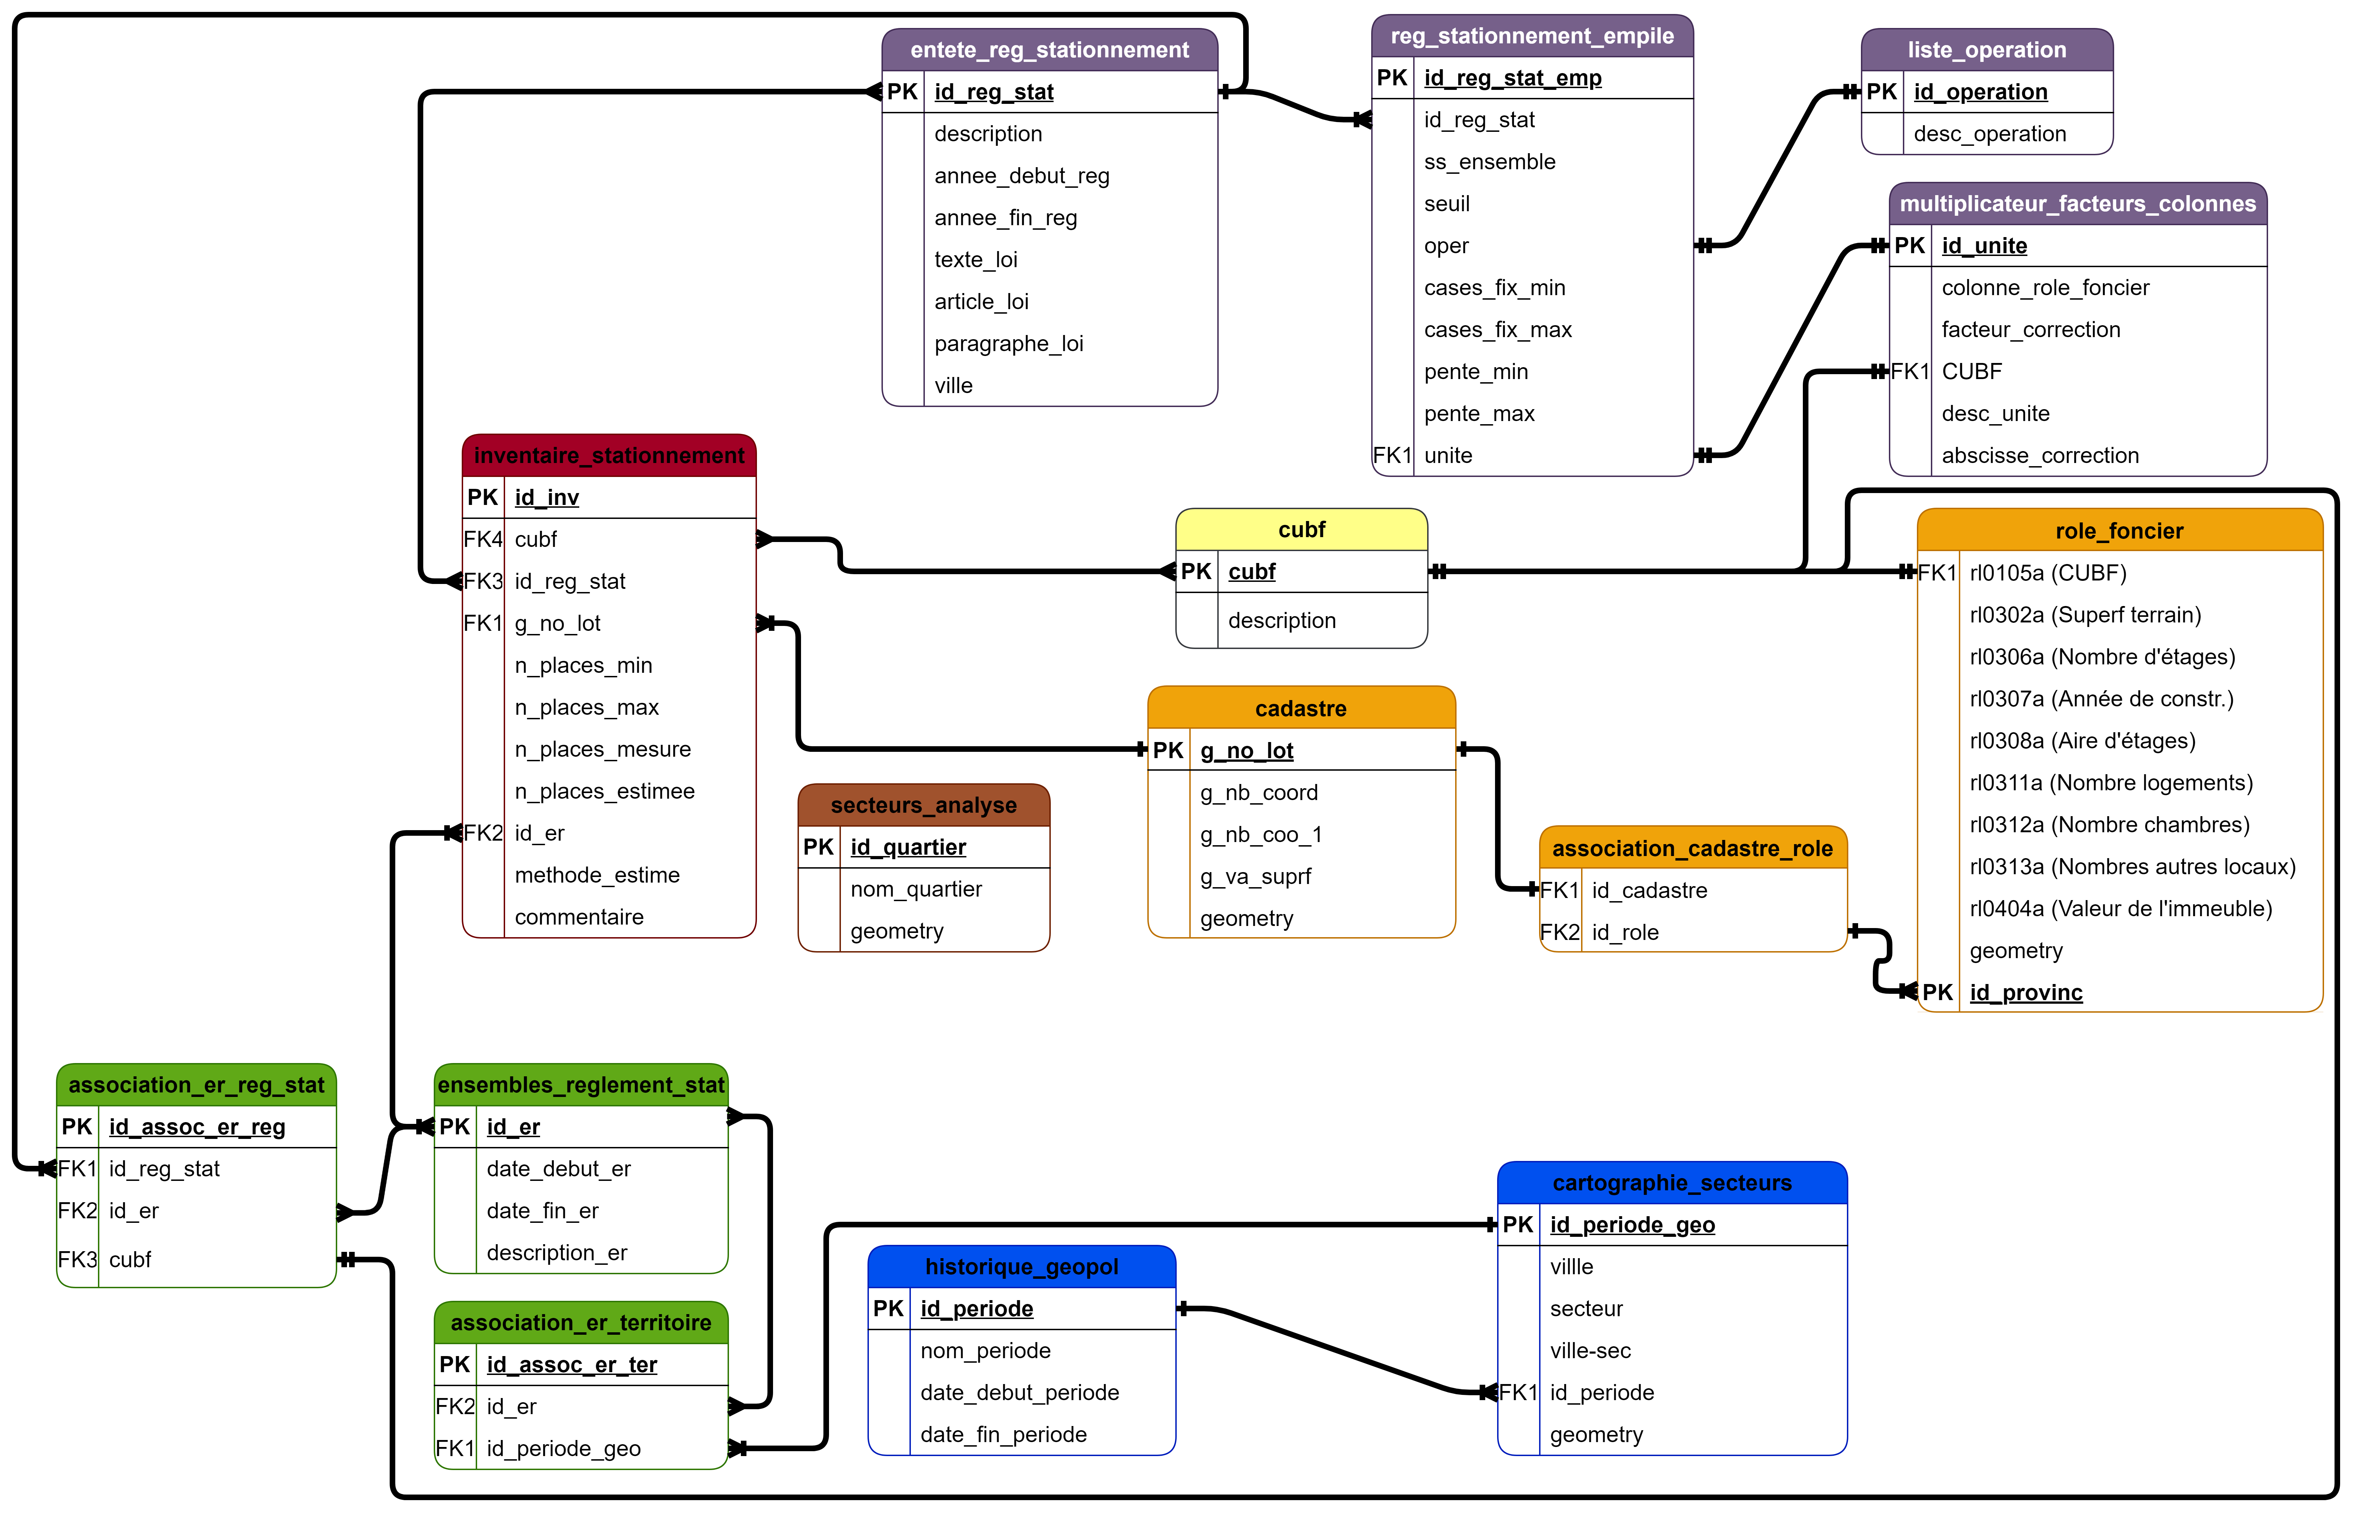
\includegraphics[trim={85cm 0 42.5cm 112.5cm}, clip, width=15cm]{dia/ERD_stationnement_propre.png}
        \caption{Structure de données pour l'historique géopolitique}\label{fig:offstreet_db_erd_history}
    \end{figure}
    \FloatBarrier
    
    \subsection{Structure de données représentant les règlements} 
        Puisque la formulation des règlements peut être relativement complexe. Deux tables sont utilisées. La première \underline{entete\_reg\_stationnement} représente les données administratives communes, tandis que \underline{reg\_stationnement\_empile} entrepose la représentation mathématique des règlements. Les champs de la table \underline{entete\_reg\_stationnement} sont énumérés dans le tableau \ref{tab:definition_entete_reg_stationnement}.  \par
        \begin{table}[h]
            \centering
            \begin{tabular}{m{0.2\textwidth}|m{0.4\textwidth}m{0.15\textwidth}m{0.075\textwidth}}
                \hline
                Nom champ & Description & Type de données & CP/CS  \\
                \hline
                id\_reg\_stat & Clé primaire  & Serial & CP \\ 
                description & Description & Texte & \\ 
                annee\_debut\_reg & Année où le règlement est entré en vigueur & Entier & \\ 
                annee\_fin\_reg & Année d'abrogation du règlement & Entier & \\ 
                texte\_loi & Texte de loi où le règlement est introduit & Texte & \\
                article\_loi & Article de loi détaillant le règlement & Texte & \\
                paragraphe\_loi &  Paragraphe de la loi détaillant le règlement & Texte & \\ 
                ville & Ville où le règlement s'applique & Texte & \\
                
                \hline
            \end{tabular}
            \caption{Colonnes pour la table \underline{entete\_reg\_stationnement}}
            \label{tab:definition_entete_reg_stationnement}
        \end{table}
        La formulation mathématique du nombre de places requises est entreposée dans la table \underline{reg\_stat\_empile}. Chaque règlement peut être divisé en sous-ensembles si le règlement propose plusieurs méthodes de calcul. L'hypothèse fondamentale est que les règlements sont essentiellement des combinaisons de formules mathématiques linéaires.\par
        \begin{table}[h]
           \centering
           \begin{tabular}{m{0.2\textwidth}|m{0.4\textwidth}m{0.15\textwidth}m{0.075\textwidth}}
                \hline
                Nom champ & Description & Type de données & CP/CS  \\
                \hline
                id\_reg\_stat\_emp & Clé primaire  & Serial & CP \\ 
                id\_reg\_stat & Référence à l'entête du règlement & Entier & CS \\ 
                ss\_ensemble & Sous-ensemble pour la ligne & Entier & \\ 
                seuil & Seuil inférieur de validité du règlement & Entier & \\ 
                oper  & Opération utilisée  & Entier & \\
                cases\_fix\_min & Ordonnée à l'origine pour le minimum & Réel & \\
                cases\_fix\_max & Ordonnée à l'origine pour le maximum  & Réel & \\ 
                pente\_min & Pente de la droite pour le minimum & Réel & \\
                pente\_max & Pente de la droite pour le maximum & Réel & \\
                unite & Unité à utiliser. Cf tableau \ref{tab:operations_table} & Entier & \\
                \hline
           \end{tabular}
           \caption{Colonnes pour la table \underline{reg\_stat\_empile}}
           \label{tab:definition_reg_stat_emp}
        \end{table}    
        \clearpage
        Les valeurs possibles des opérations sont listées au tableau \ref{tab:operations_table}. Il est important de noter que les opérations 1 et 4 sont implémentées à l'intérieur d'un même sous-ensemble, alors que les opérations 3-6 sont implémentées entre deux sous-ensembles.\par
        \begin{table}[h]
            \centering
            \begin{tabular}{cl}
                 \hline
                 id\_operation & desc\_operation  \\ \hline
                 1 & + (absolu)\\
                 3 & ou (plus contraignant) \\
                 4 & changement critère au dela seuil (>=)\\
                 6 & ou simple \\ \hline
            \end{tabular}
            \caption{Entrées dans la table liste\_operations}
            \label{tab:operations_table}
        \end{table}
        Le champ unité de la table \underline{reg\_stat\_empile} est la clé primaire pour la table \underline{multiplicateur\_facteurs\_colonnes}. Le tableau \ref{tab:definition_unite} en décrit les champs.\par
        \begin{table}[h]
           \centering
           \begin{tabular}{m{0.25\textwidth}|m{0.4\textwidth}m{0.1\textwidth}m{0.075\textwidth}}
                \hline
                Nom champ & Description & Type de données & CP/CS  \\
                \hline
                id\_unite & Clé primaire  & Serial & CP \\  
                colonne\_role\_foncier & Colonne du rôle foncier à utiliser pour cette unité & Texte & \\
                facteur\_correction & Facteur de multiplication pour & Réel & \\
                cubf & Optionnel: facteur différent pour un CUBF spécifique & Entier & \\
                desc\_unite & Description de l'unité & Texte & \\
                \rowcolor{red}abscisse\_correction & Ordonnée à l'origine de la pente de regression & Réel &  \\
                \hline
           \end{tabular}
           \caption{Colonnes pour la table \underline{multiplicateur\_facteur\_colonne}}
           \label{tab:definition_unite}
        \end{table}   
        \clearpage
        Le tableau \ref{tab:unite_pertinentes_minimum_stat} donne  le contenu de la table multiplicateur\_facteur\_colonnes. Ce tableau permet d'associer les colonnes du rôle foncier à une unité utilisée dans les règlements. De plus, il permet de faire des conversions linéaires. On pourrait penser notamment à la conversion d'espace au sol en capacité assise pour certains établissements.\par
        \begin{table}[h]
        \centering
            \begin{tabular}{c l c c p{3cm}}
                \hline
                id\_unite & colonne\_role\_foncier & facteur\_correction & cubf & desc\_unite \\ \hline
                1 & rl0312a & 1 & S.V. & chambre\\
                2 & rl0311a & 1 & S.V. & logement \\
                4 & rl0308a & 1 & S.V. & metre carré d'étage\\
                5 & S.V. & 1 & S.V. & metre carré bureau\\
                \rowcolor{red}6 & S.V. & 1 & S.V. & metre carré salle production \\
                \rowcolor{red}7 & rl0302a & 1 & S.V. & metre carré terrain\\
                \rowcolor{red}8 & S.V. & 1 & S.V. & siège \\
                \rowcolor{red}9 & S.V. & 1 & S.V. & poste de travail \\
                \rowcolor{red}10 &S.V. & 1 & S.V. & salle \\
                \rowcolor{red}11 & S.V. & 1 & S.V. & lit \\
                \rowcolor{red}12 & S.V. & 1 & S.V. & personne \\
                \rowcolor{red}13 & S.V. & 1 & S.V. & employé \\
                \rowcolor{red}14 & S.V. & 1 & S.V. & étudiant \\
                \rowcolor{red}15 & S.V. & 1 & S.V. & médecin \\
                \rowcolor{red}16 & S.V. & 1 & S.V. & quai \\
                \rowcolor{red}17 & S.V. & 1 & S.V. & voie de service \\
                \rowcolor{red}18 & S.V. & 1 & S.V. & vert \\
                \rowcolor{red}19 & S.V. & 1 & S.V. & allee de pratique \\
                \rowcolor{red}20 & S.V. & 1 & S.V. & plateau sportif \\ \hline
            \end{tabular}
            \caption{Contenu type de la table \underline{multiplicateur\_facteur\_colonnes}}\label{tab:unite_pertinentes_minimum_stat}
        \end{table}
        \FloatBarrier
        Les étapes mathématiques pour une ligne d'un règlement de stationnement sont données aux équations \ref{eq:x_entree}, \ref{eq:places_max} et \ref{eq:places_min} si $x_{entree} \geq seuil $.
        \begin{align}
            x_{entree} &= role\_foncier[colonne\_role\_foncier] \times facteur\_correction \label{eq:x_entree}+ordonee\_correction\\
            n_{places,min} &= cases\_fix\_min + pente\_min \times x_{entree} \label{eq:places_min}\\
            n_{places,max} &= cases\_fix\_max + pente\_max \times x_{entree} \label{eq:places_max}
        \end{align}
        \clearpage
        La figure \ref{fig:offstreet_db_erd_rules} montre le schéma relationnel pour les règlements:
        \begin{figure}[!h]
            \centering
            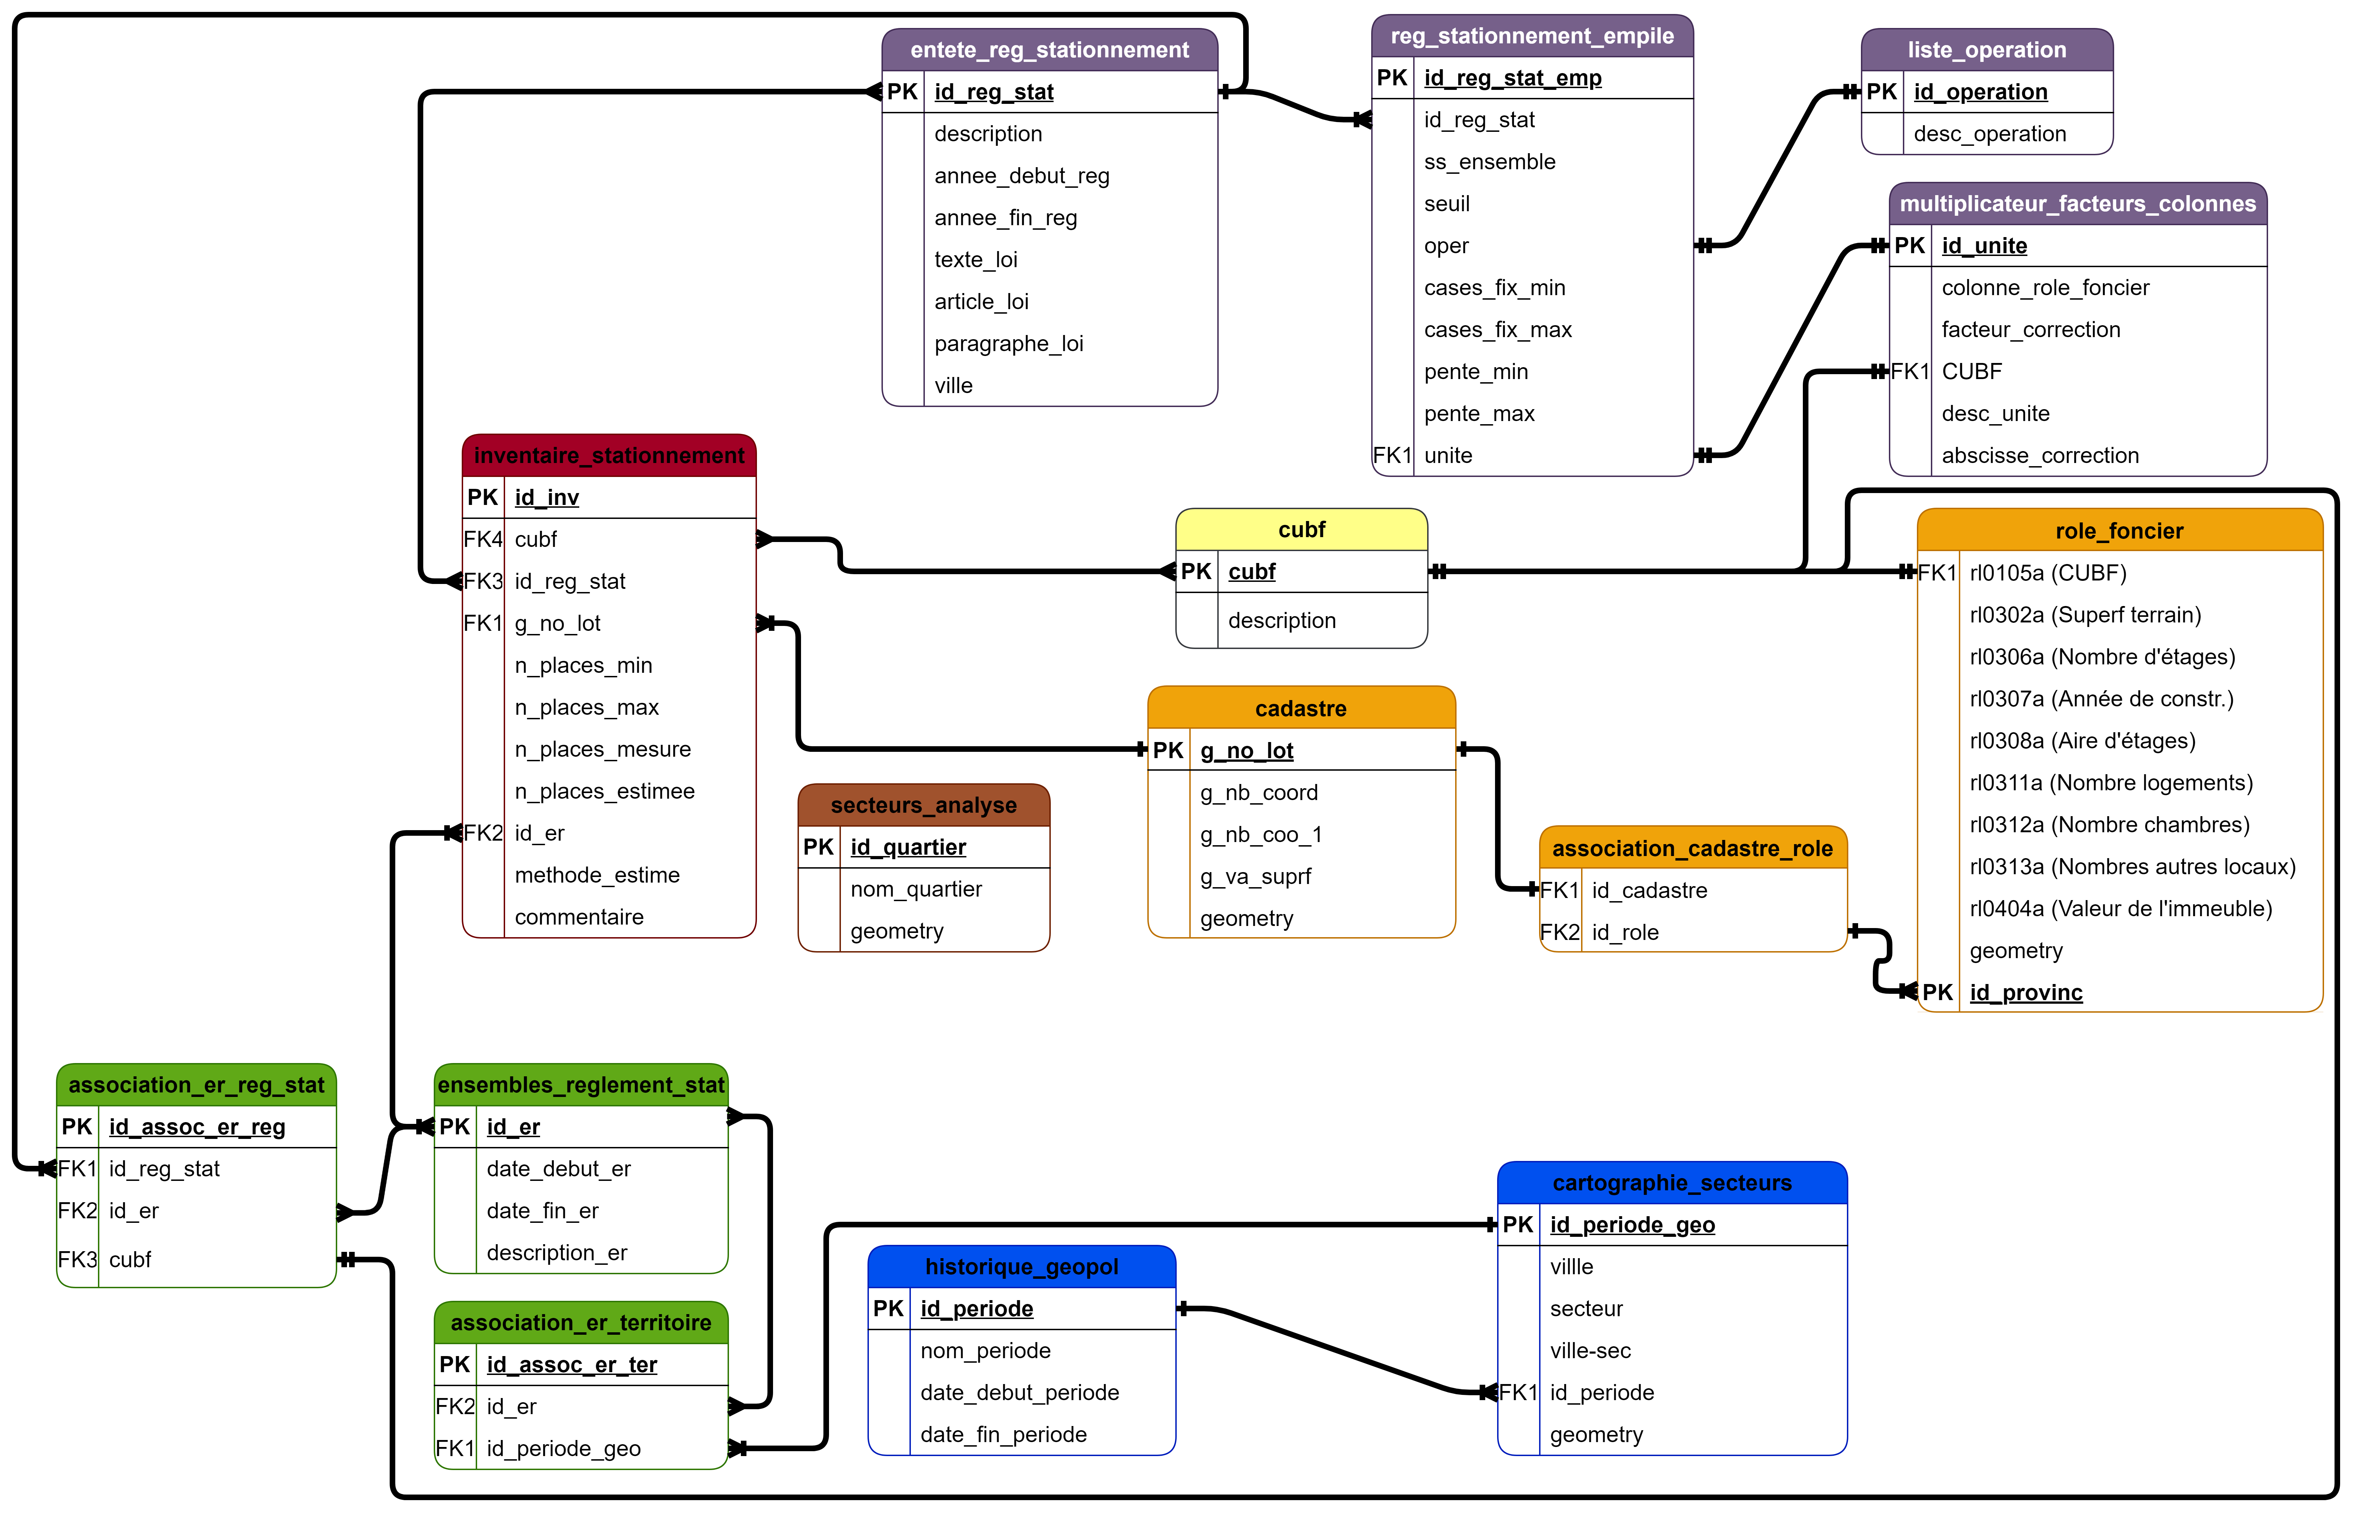
\includegraphics[trim={85cm 106.25cm 0 0cm}, clip, width=15cm]{dia/ERD_stationnement_propre.png}
            \caption{Structure de données pour les règlements}\label{fig:offstreet_db_erd_rules}
        \end{figure}
        \FloatBarrier
        \clearpage
    \subsubsection{Exemple 1: Clinique medicale} 
        Admettons un règlement qui requiert 1 place par salle de consultation  plus une place par employé plus une place par médecin ou une place par 20 mètres carrés, au plus contraignant. Les entrées dans la table reg\_stat\_empile seraient telles que montrées au tableau \ref{tab:ex_reg_stat_clinique}
        \begin{table}[h]
            \centering
            \begin{tabular}{cccccccccc}
                \hline
                \rotatebox{90}{id\_emp} & \rotatebox{90}{id\_reg\_stat} & \rotatebox{90}{ss\_ensemble} & \rotatebox{90}{seuil}  & \rotatebox{90}{oper}  & \rotatebox{90}{cases\_fix\_min}   & \rotatebox{90}{cases\_fix\_max}   & \rotatebox{90}{pente\_min}    & \rotatebox{90}{pente\_max} & \rotatebox{90}{unite}    \\ \hline
                1                       & 1                             &  1                           & 0                      &  S.V.                 & 0                                 & S.V.                              & 1                             & S.V.                       & 15                       \\
                2                       & 1                             &  1                           & 0                      &  1                    & 0                                 & S.V.                              & 1                             & S.V.                       & 13                       \\
                3                       & 1                             &  1                           & 0                      &  1                    & 0                                 & S.V.                              & 1                             & S.V.                       & 10                       \\
                4                       & 1                             &  2                           & 0                      &  3                    & 0                                 & S.V.                              & 0.05                          & S.V.                       & 4                       \\ \hline
            \end{tabular}
            \caption{Exemple règlements dans la table \underline{reg\_stat\_empile} pour une clinique médicale}
            \label{tab:ex_reg_stat_clinique}
        \end{table}
        \begin{figure}[h]
        \begin{subfigure}[t]{0.5\textwidth}
           \centering
           \begin{tikzpicture}[scale=0.8]
            \begin{axis}[
                xlabel={$N_{employes}$[-]},
                ylabel={$N_{médecin}$[-]},
                zlabel={$N_{places}$[-]},
                legend style={at={(0.5,1.25)},
    	           anchor=north,legend columns=-1}
            ]
            \addplot3[
                surf,color = blue, faceted color=black,
            ] 
            coordinates {
            (0,0,1) (0,1,2) (0,2,3)
            
            (1,0,2) (1,1,3) (1,2,4)
            
            (2,0,3) (2,1,4) (2,2,5)
            };
            \addplot3[
                surf,color = orange, faceted color=black,
            ] 
            coordinates {
            (0,0,2) (0,1,3) (0,2,4)
            
            (1,0,3) (1,1,4) (1,2,5)
            
            (2,0,4) (2,1,5) (2,2,6)
            };
            \legend{Stat min. $n_{salles}=1$,Stat min. $n_{salles}=2$}
            \end{axis} 
            \end{tikzpicture}
            \caption{Sous ensemble 1 du règlement}
        \end{subfigure}
        ~
        \begin{subfigure}[t]{0.5\textwidth}
            \centering
            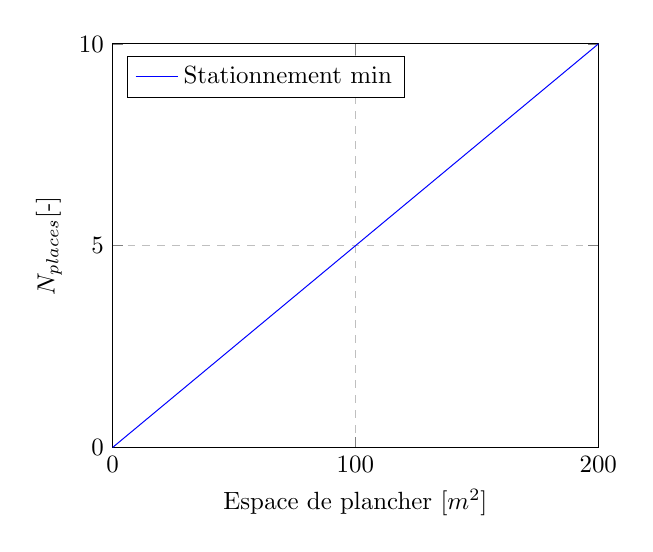
\begin{tikzpicture}[scale = 0.9]
            \begin{axis}[
                xlabel={Espace de plancher [$m^2$]},
                ylabel={$N_{places}$[-]},
                xmin=0, xmax=200,
                ymin=0, ymax=10,
                xtick={0,100,200},
                ytick={0,5,10},
                    legend pos=north west,
                ymajorgrids=true,
                xmajorgrids=true,
                grid style=dashed,
                domain=0:1000, 
            ]
            \addplot[color=blue]{x/20};
            \legend{Stationnement min}
            \end{axis}
        \end{tikzpicture}
        \caption{Sous ensemble 2 du règlement}
        \end{subfigure}
        \caption{Exemple de règlement de stationnement pour une clinique médicale}
        \end{figure}
        \FloatBarrier
        \clearpage
    \subsubsection{Exemple 2: Logements} 
        Dans le cas d'un logement, les règlements changent souvent en fonction du nombre de logements au sein d'un même bâtiment. Dans ce cas hypothétique, le requis serait d'une case par logement pour des bâtiments de moins de 4 logements, 1.5 cases par logement pour les bâtiments entre 4 et 7 logements et 1.25 case par logement pour tout bâtiment de 8 logements ou plus. Dans ce cas, les entrées à la table seraient telles que montrées au tableau
        \begin{table}[h]
            \centering
            \begin{tabular}{cccccccccc}
                \hline
                \rotatebox{90}{id\_emp} & \rotatebox{90}{id\_reg\_stat} & \rotatebox{90}{ss\_ensemble} & \rotatebox{90}{seuil}  & \rotatebox{90}{oper}  & \rotatebox{90}{cases\_fix\_min}   & \rotatebox{90}{cases\_fix\_max}   & \rotatebox{90}{pente\_min}    & \rotatebox{90}{pente\_max} & \rotatebox{90}{unite}    \\ \hline
                5                       & 2                             &  1                           & 0                      &  S.V.                 & 0                                 & S.V.                              & 1                             & S.V.                       & 2                       \\
                6                       & 2                             &  1                           & 4                      &  4                    & 0                                 & S.V.                              & 1.5                           & S.V.                       & 2                       \\
                7                       & 2                             &  1                           & 8&  4                    & 0                                 & S.V.                              & 1.25                          & S.V.                       & 2                       \\ \hline
            \end{tabular}
            \caption{Exemple règlements dans la table \underline{reg\_stat\_empile} pour le logement}
            \label{tab:ex_reg_logement}
        \end{table}
         \begin{figure}[h]
           \centering
            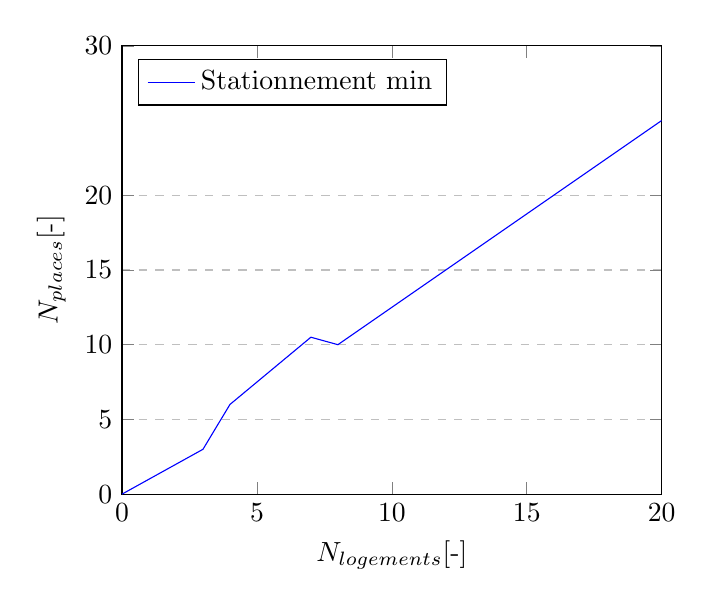
\begin{tikzpicture}[scale=1.0]
                \begin{axis}[
                    xlabel={$N_{logements}$[-]},
                    ylabel={$N_{places}$[-]},
                    xmin=0, xmax=20,
                    ymin=0, ymax=30,
                    xtick={0,5,10,15,20},
                    ytick={0,5,10,15,20,30},
                    legend pos=north west,
                    ymajorgrids=true,
                    grid style=dashed,
                ]
                \addplot[
                        color=blue
                        ]
                     coordinates {
                        (0,0)(3,3)(4,6)(5,7.5)(6,9)(7,10.5)(8,10)(10,12.5)(15,18.75)(20,25)
                    };
        
                \legend{Stationnement min}
                \end{axis}
            \end{tikzpicture}
        \caption{Exemple de règle de stationnement pour logement}
        \end{figure}
        \FloatBarrier
        \clearpage
    \subsubsection{Exemple 3: Lieux d'assemblée} 
        Dans le cas de lieux d'assemblée, les requis peuvent être exprimés en fonction du nombre de sièges ou en fonction de l'espace au sol. Dans notre cas hypothétique, le requis serait un minimum d'une place par 7 sièges jusqu'à 800 sièges et d'un minimum de 1 place par 9 sièges pour toute place au-delà de 800 sièges. Un maximum  d'une place par 5 sièges est applicable au-delà de 500 sièges. Quand il n'y a pas de sièges, un requis d'une places par 10 mètres carrés est applicable sans maximum.
        \begin{table}[h]
            \centering
            \begin{tabular}{cccccccccc}
                \hline
                \rotatebox{90}{id\_emp} & \rotatebox{90}{id\_reg\_stat} & \rotatebox{90}{ss\_ensemble} & \rotatebox{90}{seuil}  & \rotatebox{90}{oper}  & \rotatebox{90}{cases\_fix\_min}   & \rotatebox{90}{cases\_fix\_max}   & \rotatebox{90}{pente\_min}    & \rotatebox{90}{pente\_max} & \rotatebox{90}{unite}    \\ \hline
                8                       & 3                             &  1                           & 0                      &  S.V.                 & 0                                 & S.V.                              & 0.142857                      & S.V.                       & 8                       \\
                9                       & 3                             &  1                           & 500                    &  4                    & 0                                 & 0                                 & 0.142857                      & 0.2                        & 8                       \\
                10                      & 3                             &  1                           & 800                    &  4                    & 25.396825                         & 0                                 & 0.111111                      & 0.2                        & 8                       \\
                11                      & 3                             &  2                           & 0                      &  6                    & 0                                 & S.V.                              & 0.1                           & S.V.                       & 4                       \\\hline
            \end{tabular}
            \caption{Exemple règlements dans la table \underline{reg\_stat\_empile} pour un lieu d'assemblée}
            \label{tab:ex_reg_lieu_assemblee}
        \end{table}
        \begin{figure}[h]
            \begin{subfigure}[t]{0.5\textwidth}
            \centering
                \begin{tikzpicture}[scale = 0.9]
                    \begin{axis}[
                        xlabel={$N_{sièges}$[-]},
                        ylabel={$N_{places}$[-]},
                        xmin=0, xmax=1000,
                        ymin=0, ymax=200,
                        xtick={0,200,400,600,800,1000},
                        ytick={0,50,100,150,200},
                            legend pos=north west,
                        ymajorgrids=true,
                        grid style=dashed,
                    ]
                
                        \addplot[
                            color=blue
                            ]
                            coordinates {
                            (0,0)(500,71.4285)(800,114.2856)(1000,136.507938)
                            };
                        \addplot[
                            color = red
                            ]
                            coordinates{
                                (500,100)(1000,200)
                            };
                        \legend{Stationnement min, Stationnement max}
                    \end{axis}
                \end{tikzpicture}
                \caption{Avec sièges}
            \end{subfigure}
            \begin{subfigure}[t]{0.5\textwidth}
                \centering
                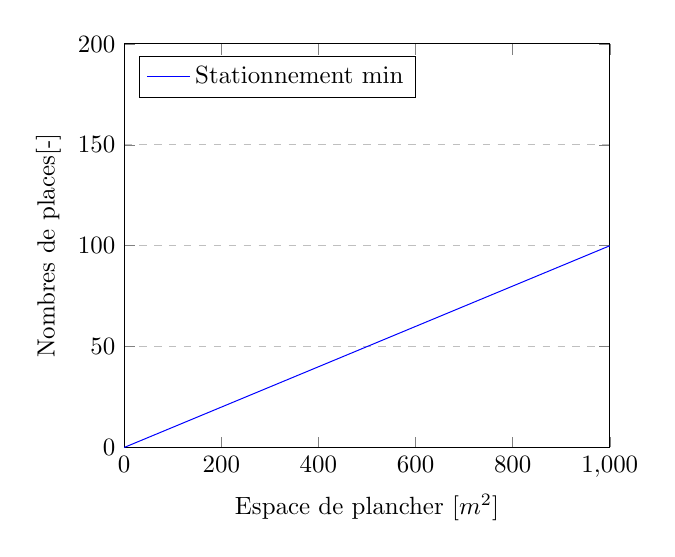
\begin{tikzpicture}[scale = 0.9]
                \begin{axis}[
                    xlabel={Espace de plancher [$m^2$]},
                    ylabel={Nombres de places[-]},
                    xmin=0, xmax=1000,
                    ymin=0, ymax=200,
                    xtick={0,200,400,600,800,1000},
                    ytick={0,50,100,150,200},
                        legend pos=north west,
                    ymajorgrids=true,
                    grid style=dashed,
                ]
                    \addplot[
                        color=blue
                        ]
                    coordinates {
                    (0,0)(500,50)(800,80)(1000,100)
                    };
                    \legend{Stationnement min}
                \end{axis}
            \end{tikzpicture}
            \caption{Sans sièges}
        \end{subfigure}
        \captionsetup{justification=centering}
        \caption{Exemple de règle de stationnement pour lieux d'assemblée}
        \end{figure}
        \FloatBarrier
    \subsection{Structure de données représentant l'ensemble des règlements applicables sur un territoire à une période donnée} \label{sec:ensembles_association}
        Cette section va introduire le schéma relationnel de données qui permet d'associer un ensemble de règlements à un territoire pour une période donnée. Trois tables sont utilisées pour représenter la variation spatio-temporelle de la réglementation: \underline{ensembles\_reglements\_stat}, \underline{cubf}, \underline{association\_er\_reg\_stat} et \underline{assoc\_er\_territoire}.\par
        \underline{ensembles\_reglements\_stat} est une entête pour chaque ensemble de règlements. Le tableau \ref{tab:definition_er} montre les colonnes de la table \underline{ensembles\_reglements\_stat}. \par
        \begin{table}[h]
           \centering
           \begin{tabular}{m{0.25\textwidth}|m{0.4\textwidth}m{0.1\textwidth}m{0.075\textwidth}}
                \hline
                Nom champ & Description & Type de données & CP/CS  \\
                \hline
                id\_er & Clé primaire  & Serial & CP \\  
                date\_debut\_er & Année où l'ensemble de règlements entre en vigueur & Entier & \\
                date\_fin\_er & Année où l'ensemble de règlements est abrogé& Entier & \\
                description\_er & Description à la discrétion de l'utilisateur & Texte & \\
                \hline
           \end{tabular}
           \caption{Colonnes pour la table \underline{ensembles\_reglement\_stat}}
           \label{tab:definition_er}
       \end{table}   
       La table \ac{CUBF} reproduit les données du gouvernement sur le code d'utilisation du bien-fonds, associant un numéro à une description sommaire. Toutes les entrées dans le rôle foncier se voient attribuer un code à 4 chiffres entre 1000 et 9999 qui définit l'usage prédominant sur la propriété. En plus de ces codes. La table entreposée dans le cadre de ce projet contient les entêtes de chaque section (e.g. 1 - logement, 15 - Habitation en commun, 154 - Maison de retraite ou orphelinat, 1542 - Orphelinat). La description des colonnes de la table \underline{cubf} est donnée au tableau \ref{tab:definition_cubf}. \par
        \begin{table}[h]
           \centering
           \begin{tabular}{m{0.25\textwidth}|m{0.4\textwidth}m{0.1\textwidth}m{0.075\textwidth}}
                \hline
                Nom champ & Description & Type de données & CP/CS  \\
                \hline
                cubf & Code d'utilisation du bien-fonds & Entier & CP \\  
                description & Description de l'utilisation du sol & Texte & \\
                \hline
           \end{tabular}
           \caption{Colonnes pour la table \underline{cubf}}
           \label{tab:definition_cubf}
        \end{table}   
       \clearpage
        \underline{association\_er\_reg\_stat} permet de faire l'association entre les \ac{CUBF}, les ensembles de règlements et les règlements décrits à la section précédente. Le tableau \ref{tab:definition_association_er_reg_stat} montre les colonnes de cette table.\par
        \begin{table}[h]
           \centering
           \begin{tabular}{m{0.25\textwidth}|m{0.4\textwidth}m{0.1\textwidth}m{0.075\textwidth}}
                \hline
                Nom champ & Description & Type de données & CP/CS  \\
                \hline
                id\_assoc\_er\_reg & Clé primaire de la table & Entier & CP \\  
                id\_reg\_stat & Identifiant du règlement à appliquer & Entier & CS \\
                cubf & \ac{CUBF} au(x)quel(s) on doit appliquer le règlement & Entier & CS\\
                id\_er & Ensemble de règlement auquel appartient l'association & Entier & CS\\
                \hline
           \end{tabular}
           \caption{Colonnes pour la table \underline{association\_er\_reg\_stat}}
           \label{tab:definition_association_er_reg_stat}
        \end{table}   
        \FloatBarrier
       
        La table \underline{association\_er\_territoire} est nécessaire pour associer les territoires aux ensembles de règlements. Le tableau \ref{tab:definition_association_er_territoire} montre les colonnes de la table.
        \begin{table}[h]
           \centering
           \begin{tabular}{m{0.25\textwidth}|m{0.4\textwidth}m{0.1\textwidth}m{0.075\textwidth}}
                \hline
                Nom champ & Description & Type de données & CP/CS  \\
                \hline
                id\_assoc\_er\_ter & Clé primaire de la table & Entier & CP \\  
                id\_er & Identifiant de l'ensemble de règlements à appliquer & Entier & CS \\
                id\_periode\_geo & Identifiant du territoire auquel s'applique l'ensemble de règlements & Entier & CS\\
                \hline
           \end{tabular}
           \caption{Colonnes pour la table \underline{association\_er\_territoire}}
           \label{tab:definition_association_er_territoire}
        \end{table}   
        La figure \ref{fig:offstreet_db_erd_rulesets} montre les tables de la base de données qui permettent de définir un ensemble de règlements. Notons que la table cubf est visible à la Figure \ref{fig:offstreet_db_erd_input_data}.
        \begin{figure}[h]
            \centering
            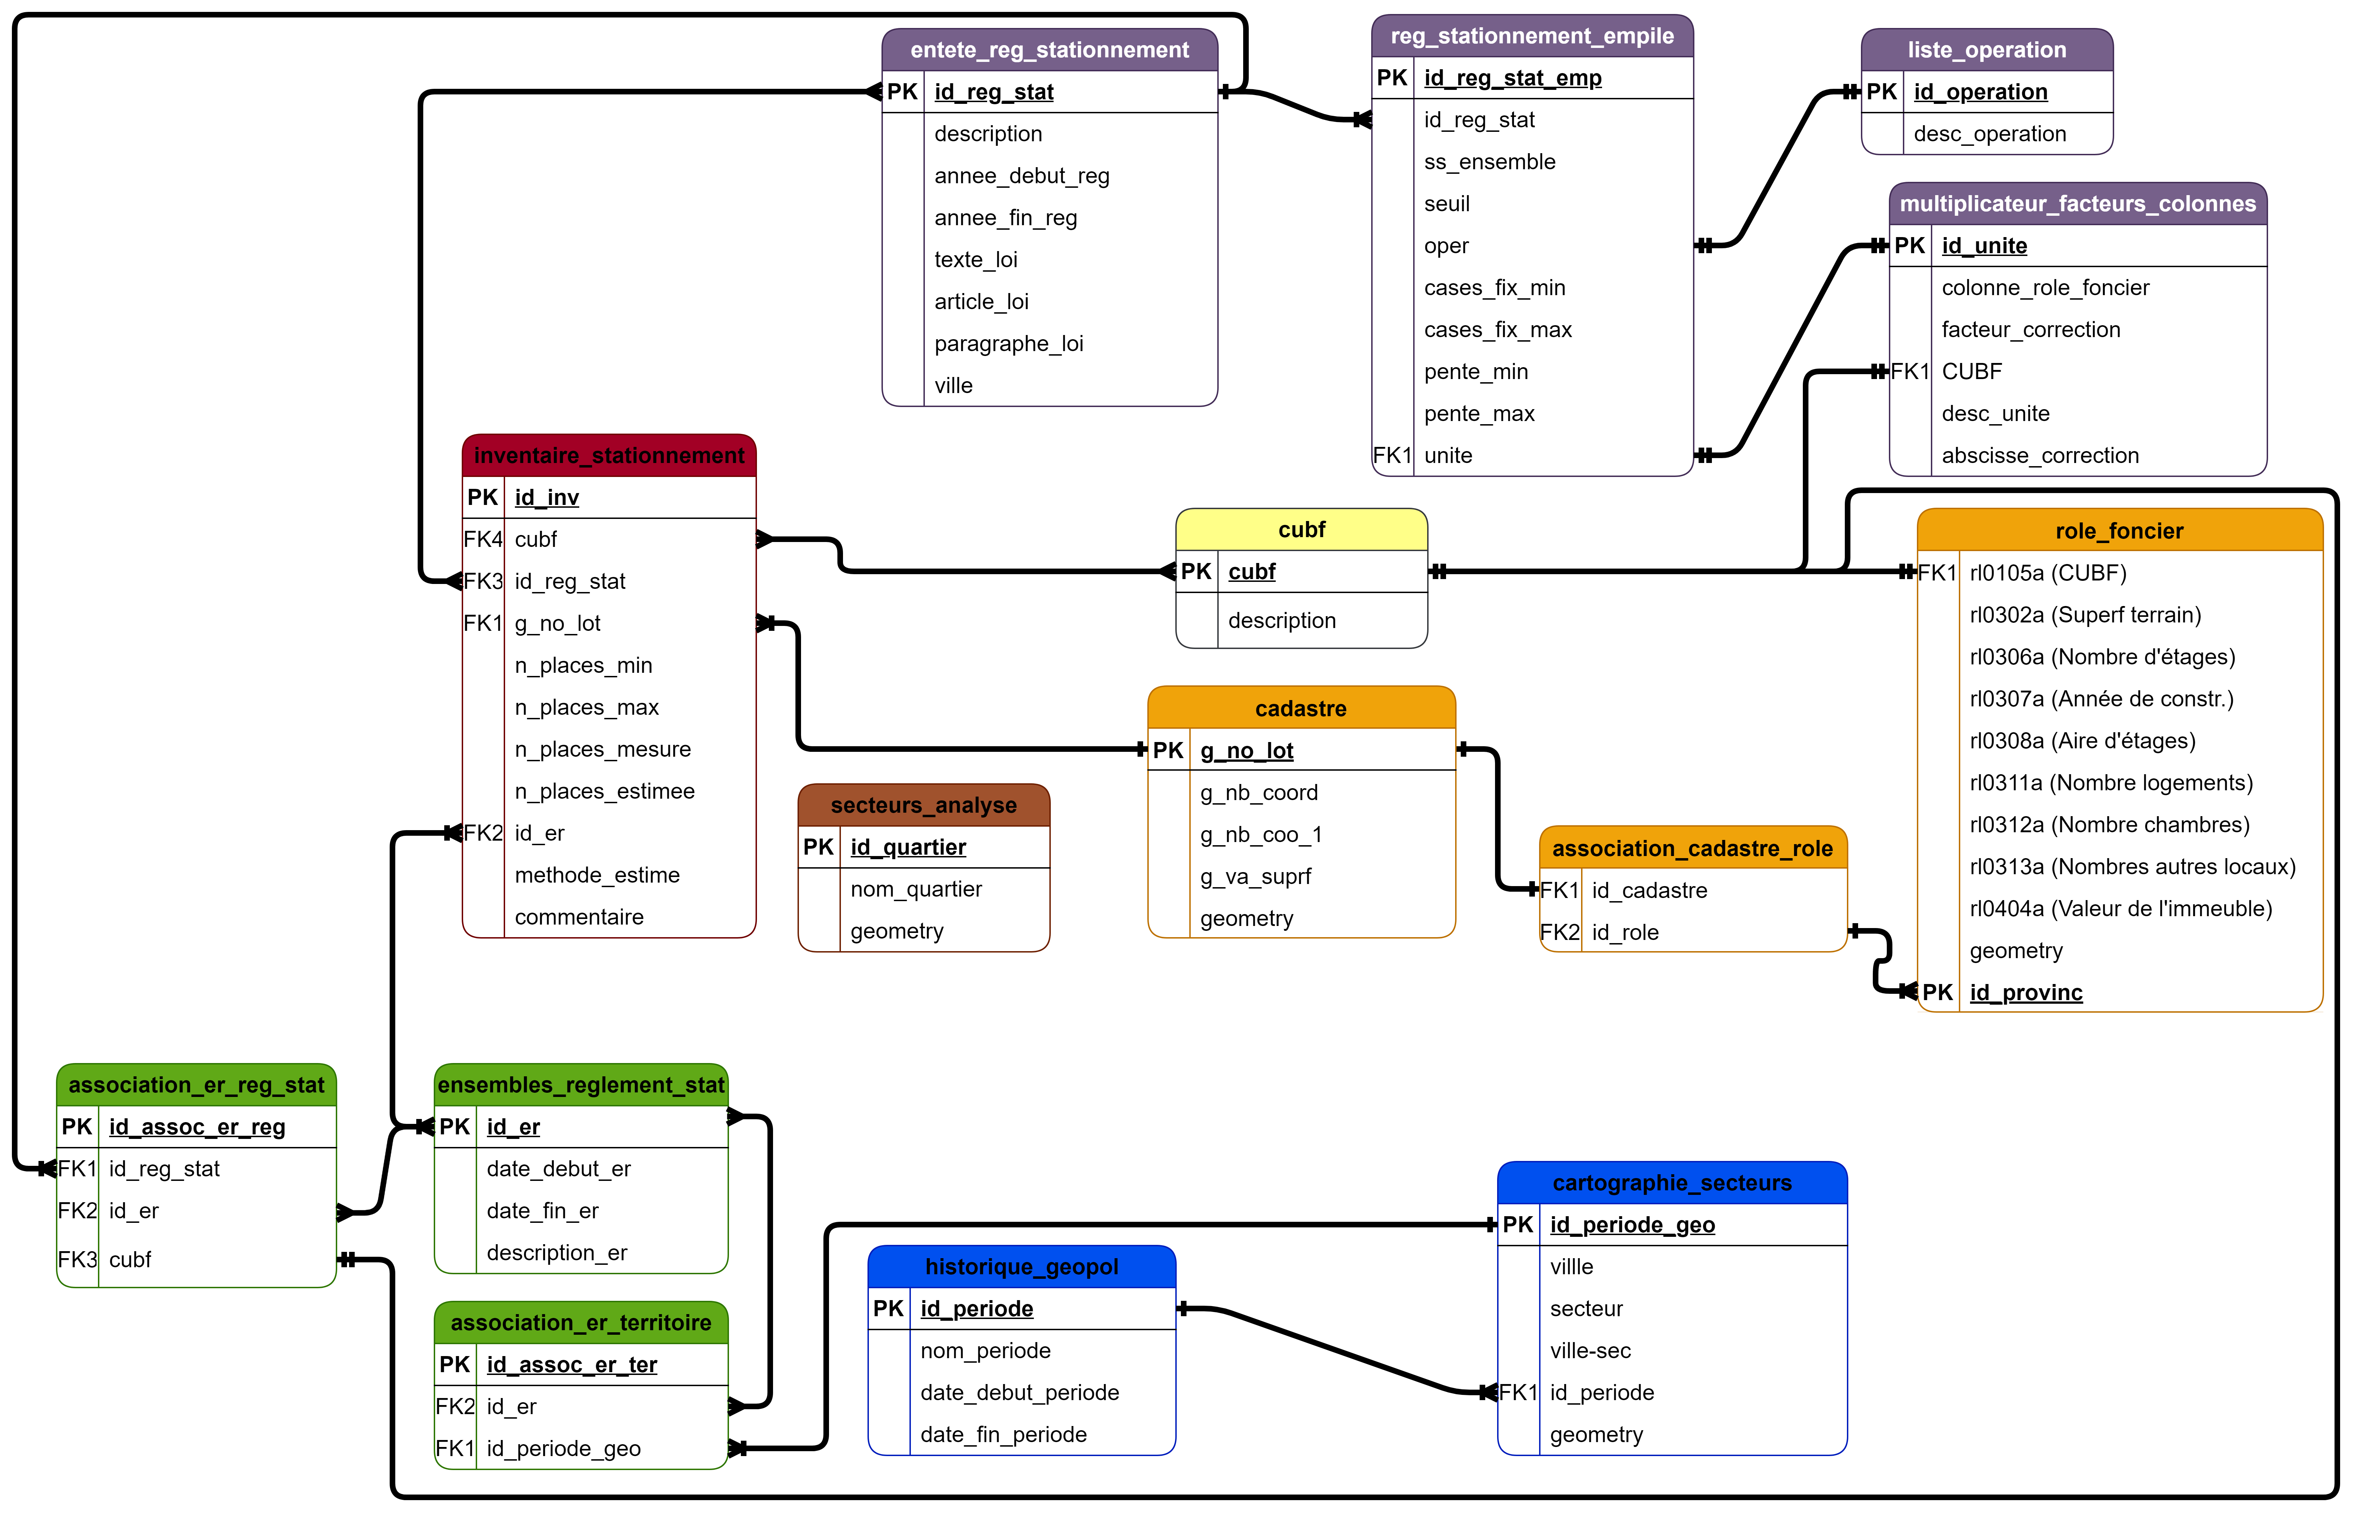
\includegraphics[trim={0 0 155cm 105cm},clip,width=15cm]{dia/ERD_stationnement_propre.png}
            \caption{Schéma relationnel pour la définition d'ensembles de règlements et leur association au territoire}
            \label{fig:offstreet_db_erd_rulesets}
        \end{figure}
        \FloatBarrier
        \subsubsection{Convention pour les règles d'association de règlement}\label{sec:reg_association}
        Par convention, toute entrée dans la table \underline{association\_er\_reg\_stat} qui s'applique à un nombre de moins de quatre chiffres s'appliquera à un ensemble plus grand. Ainsi:
        \begin{itemize}
            \item Associer 1 à un règlement verra l'ensemble des \ac{CUBF} entre 1000 et 1999 associés à cette règle
            \item Associer 15 à un règlement verra l'ensemble des \ac{CUBF} entre 1500 et 1599 associés à cette règle
            \item Associer 154 à un règlement verra l'ensemble des \ac{CUBF} entre 1540 et 1549 associés à cette règle
        \end{itemize}
        La règle la plus détaillée (avec le plus grand nombre de chiffres) aura donc préséance en cas de conflits. À minima, une entrée sera requise pour les entrées 1 à 9 pour assurer une couverture réglementaire sur l'ensemble des \ac{CUBF}.\par
        \subsubsection{Convention pour les années}
        Pour représenter la variabilité des règlements au travers du temps, des dates de validité sont mises en place sur plusieurs objets. Certains règlements ou territoires sont représentés sans date de début pour capturer tous les bâtiments construits avant une certaine date. D'autre part, il est nécessaire de représenter des règlements qui sont encore valides et n'ont donc pas de date d'abrogration. La convention suivante est donc appliquée sur les dates:
        \begin{itemize}
            \item Les règlements, ensembles de règlements ou territoires n'ayant pas de date de début capturent les entrées du rôle ayant été construits avant la date de fin desdits items.
            \item Les règlements, ensembles de règlements ou territoires n'ayant pas de date de fin capturent les entrées du rôle ayant été construits après la date de début des dits items jusqu'à aujourd'hui
        \end{itemize}
    \subsection{Structure des données cadastrales et de taxation foncière utilisées pour l'étude}
        Les données de départ sont le rôle foncier brut ainsi que le cadastre représentés dans les tables \underline{cadastre} et \underline{role\_foncier}. Le tableau \ref{tab:definition_role_foncier} donne une définition des colonnes pertinentes à ce mémoire. Ces tables ont cependant d'autres colonnes qui ne sont pas nécessairement pertinentes aux activités de ce mémoire. Cette section en détaillera seulement une partie. Le tableau \ref{tab:definition_role_foncier} montre les colonnes pertinentes dans le rôle foncier. Les descriptions sont tirées de \textcite{gouvernement_du_quebec_donnees_2022}.\par
        \begin{table}[h]
           \centering
           \begin{tabular}{m{0.25\textwidth}|m{0.4\textwidth}m{0.1\textwidth}m{0.075\textwidth}}
                \hline
                Nom champ & Description & Type de données & CP/CS  \\
                \hline
                id\_provinc & Clé primaire de la table & Texte & CP \\  
                rl0105a & Utilisation prédominante de l'unité d'évaluation & Entier & CS  \\
                rl0302a & Superficie du terrain en mètres carrés & Réel & \\ 
                rl0306a & Nombre d'étages & Entier & \\
                rl0307a & Année de construction & Entier & \\
                rl0308a & Aire d'étages en mètres carrés & Réel & \\
                rl0311a & Nombre de logements dans l'unité d'évaluation & Entier &  \\
                rl0312a & Nombre de chambres locatives & Entier & \\
                rl0313a & Nombre de locaux non-résidentiels & Entier & \\
                rl0404a & Valeur de l'immeuble(terrain + bâtiment) & Entier & \\
                geometry & Géométrie (Point) du rôle foncier & Géométrie & \\
                \hline
           \end{tabular}
           \caption{Colonnes pour la table \underline{role\_foncier}}
           \label{tab:definition_role_foncier}
        \end{table}   
        La table \underline{association\_cadastre\_role} associe le cadastre avec le rôle foncier. En premier lieu, une jointure géométrique a été complétée et sauvegardée. Cette opération est onéreuse et l'utilisation d'une table plutôt que de refaire la requête est plus efficace. D'autre part, cette méthodologie peut permettre de faire des associations plus complexes si une entrée au rôle couvre plusieurs entrées cadastrales. \par
        Ceci est différent de l'approche utilisée par la chaire, où les points du cadastre sont relocalisés sur l'entrée principale du bâtiment. L'approche proposée ici permet d'utiliser les données brutes issues de \textcite{gouvernement_du_quebec_manuel_2024}, sans avoir à manuellement remettre à jour les points chaque année. La clé primaire pour le cadastre est g\_no\_lot et la clé primaire pour le rôle est l'id\_provinc. Les champs de la table \underline{association\_cadastre\_role} sont données au tableau \ref{tab:definition_assoc_role_cadastre}:
        \begin{table}[h]
           \centering
           \begin{tabular}{m{0.25\textwidth}|m{0.4\textwidth}m{0.1\textwidth}m{0.075\textwidth}}
                \hline
                Nom champ & Description & Type de données & CP/CS  \\
                \hline
                g\_no\_lot & Identifiant du lot cadastral & Texte & \\
                id\_provinc & Identifiant du rôle & Texte & \\
                \hline
           \end{tabular}
           \caption{Colonnes pour la table \underline{association\_cadastre\_role}}
           \label{tab:definition_assoc_role_cadastre}
        \end{table}   
        \par
        Le tableau \ref{tab:definition_cadastre} donne les détails sur les entrées dans la table \underline{cadastre}. D'autres colonnes existent mais ne sont pas détaillées car elles ne sont pas utilisées au sein de ce mémoire.\par
        \begin{table}[!h]
           \centering
           \begin{tabular}{m{0.25\textwidth}|m{0.4\textwidth}m{0.1\textwidth}m{0.075\textwidth}}
                \hline
                Nom champ       & Description                   & Type de données   & CP/CS  \\
                \hline
                g\_no\_lot      & Identifiant du lot cadastral  & Texte             & CP\\
                g\_nb\_coord    & Longitude du centre de lot    & Réel              & \\
                g\_nb\_coo\_1   & Latitude du centre de lot     & Réel              & \\
                g\_va\_suprf    & Superficie du lot             & Réel              & \\
                geometry        & Géométrie du lot              & Géométrie         & \\
                \hline
           \end{tabular}
           \caption{Colonnes pour la table \underline{cadastre}}
           \label{tab:definition_cadastre}
        \end{table}   
        La figure \ref{fig:offstreet_db_erd_input_data} montre les tables pertinentes en intrant. Il est concevable que ces tables soient entreposées dans un serveur différent si cette méthodologie était implémentée dans un milieu municipal.
        \begin{figure}[ht!]
            \centering
            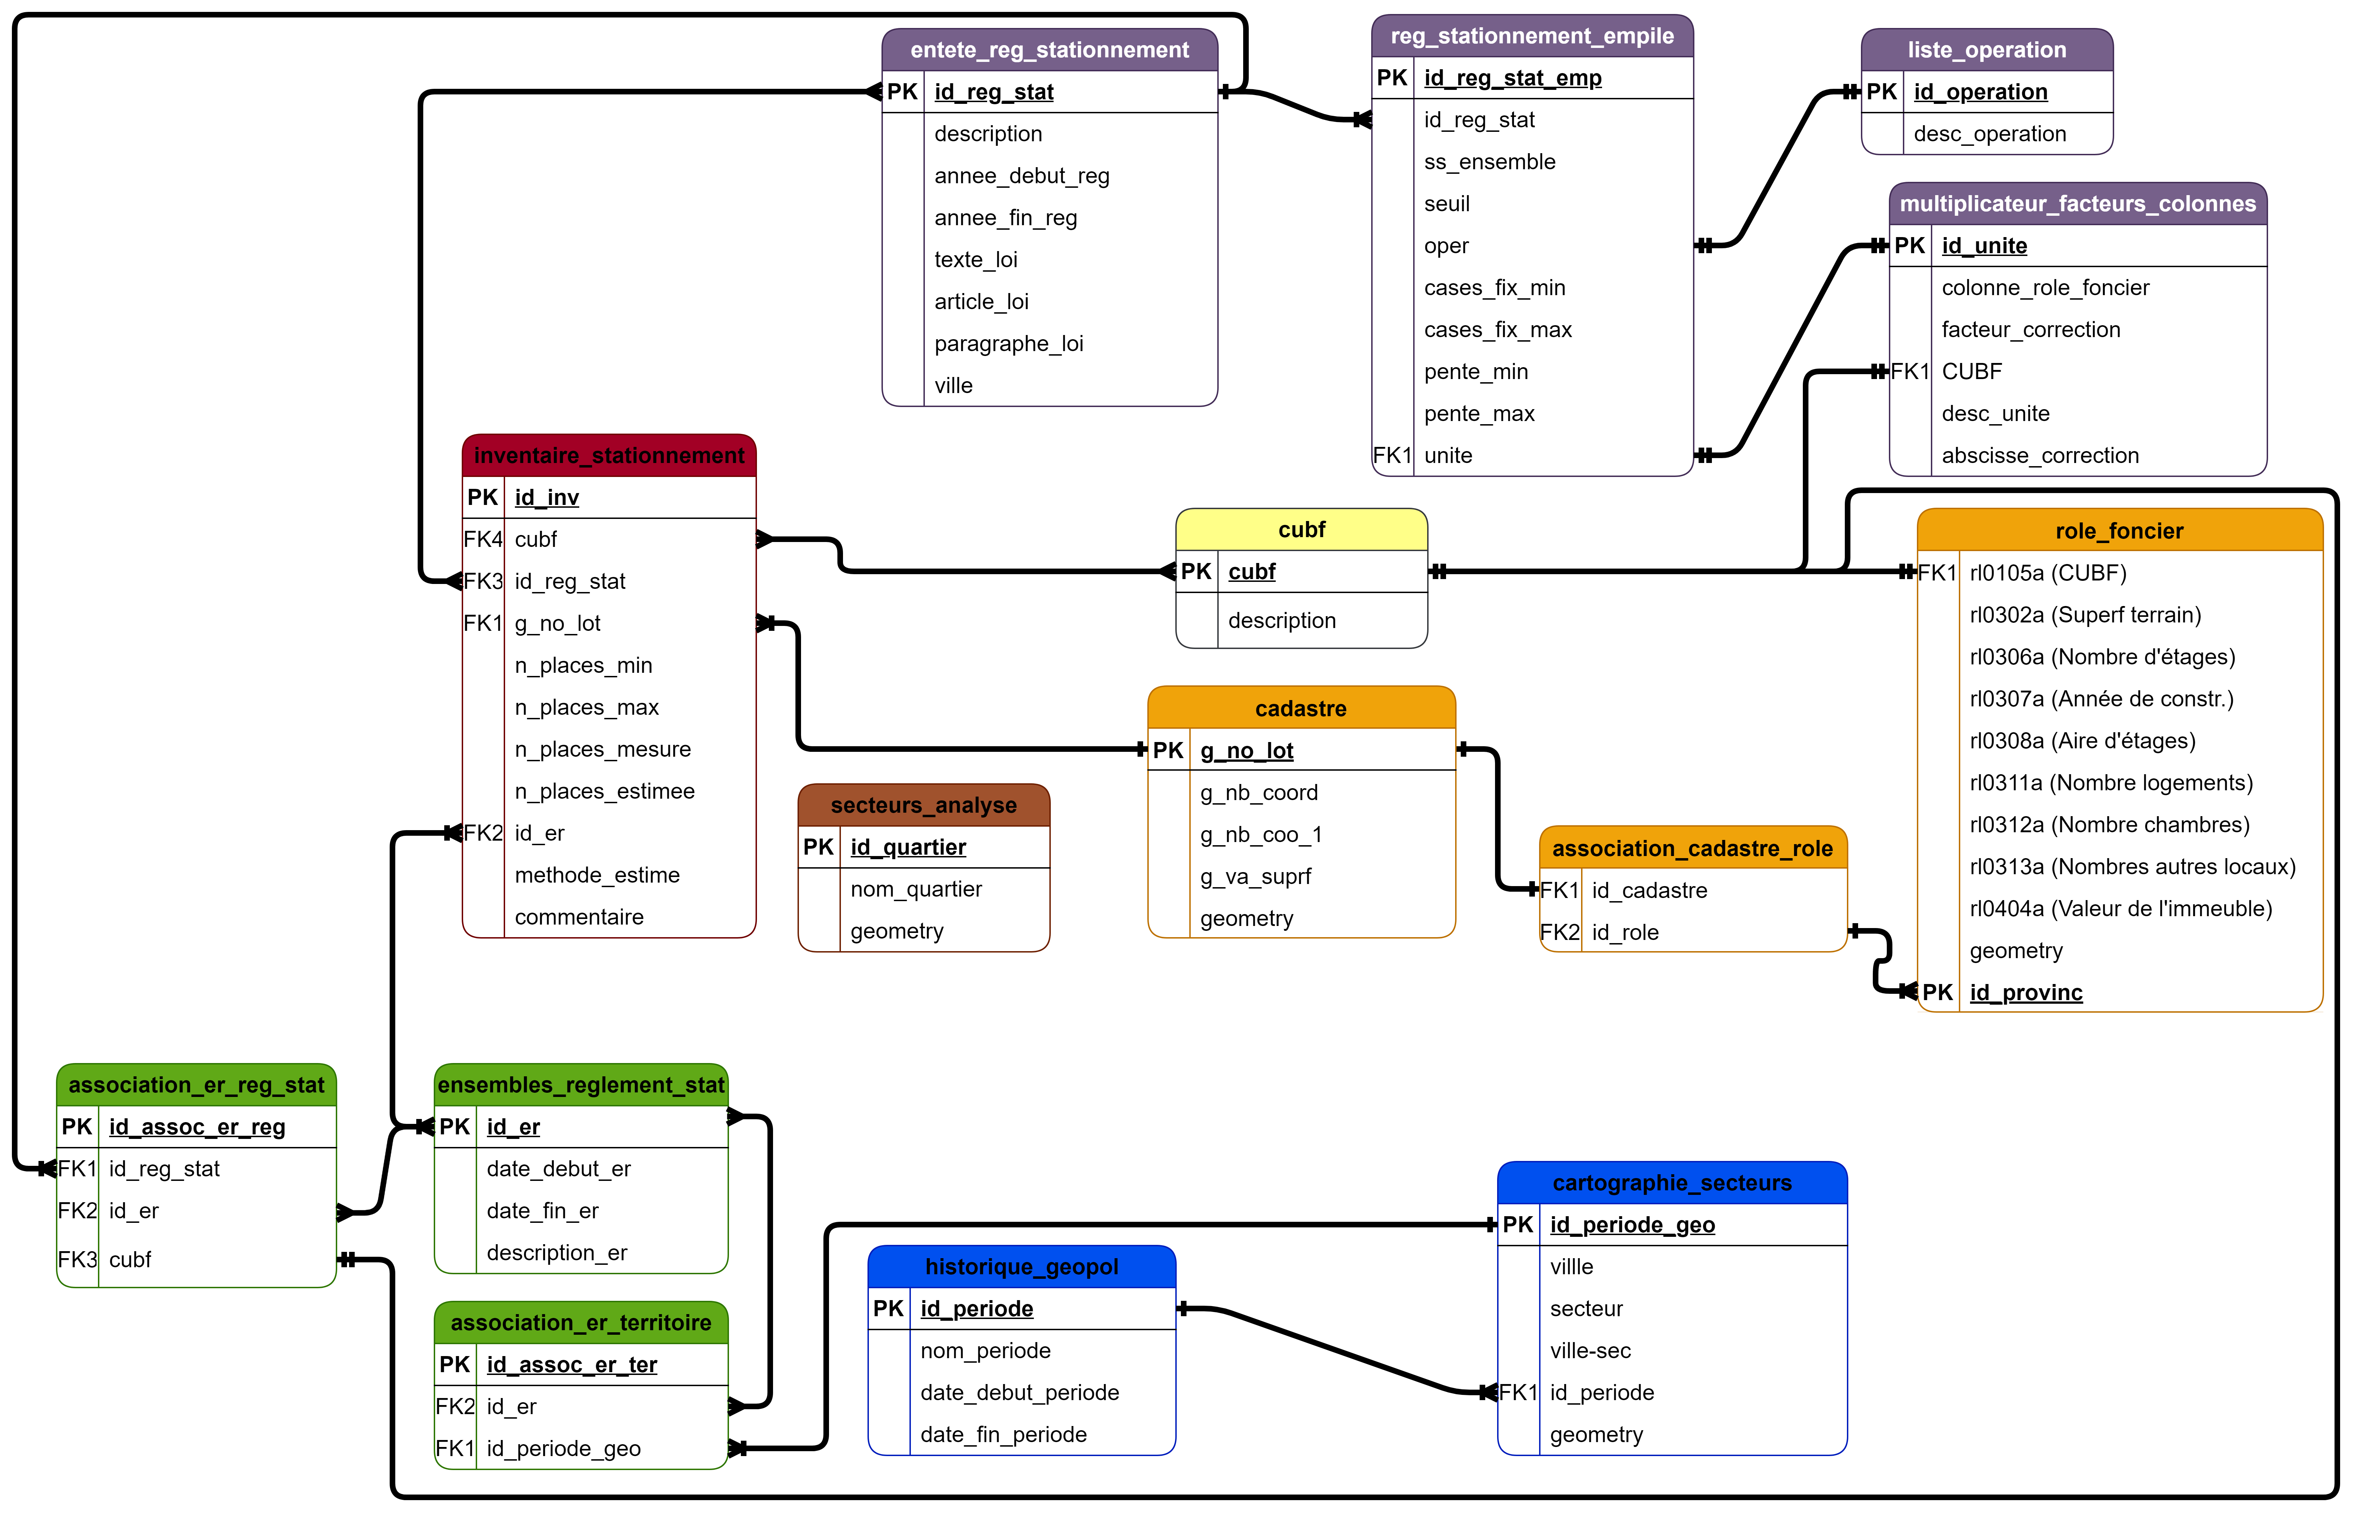
\includegraphics[trim={110cm 50cm 0cm 49cm},clip,width=15cm]{dia/ERD_stationnement_propre.png}
            \caption{Schéma relationnel pour le rôle foncier et le cadastre}
            \label{fig:offstreet_db_erd_input_data}
        \end{figure}
        \FloatBarrier
    \subsection{Structure des données représentant les secteurs d'analyse}\label{ssec:struct_donnees_sec_analyse}
        Les quartiers énumérés par la ville de Québec sont utilisés comme base de comparaison et pour diviser le territoire dans la table sec\_analyse. Les colonnes du tableau sont listées dans le tableau \ref{tab:definition_sec_analyse}.
        \begin{table}[h]
           \centering
           \begin{tabular}{m{0.25\textwidth}|m{0.4\textwidth}m{0.1\textwidth}m{0.075\textwidth}}
                \hline
                Nom champ & Description & Type de données & CP/CS  \\
                \hline
                id\_quartier & Clé primaire & Entier & CP \\
                nom\_quartier & Nom du quartier & Texte & \\
                superf\_quartier & Superficie du quartier & Réel & \\
                peri\_quartier & Périmètre du quartier & Réel & \\
                geometry & Géométrie des quartier & Géométrie & \\
                \hline
           \end{tabular}
           \caption{Colonnes pour la table \underline{sec\_analyse}}
           \label{tab:definition_sec_analyse}
        \end{table}   
        La figure \ref{fig:sec-analyse} montre les secteurs utilisés qui sont les quartiers listés dans les données ouvertes de la ville. Une autre division géographique (comme les secteurs de l'enquête OD) pourrait être substituée au besoin.
        \begin{figure}[h]
            \centering
            \includegraphics[width=0.7\linewidth]{images/secteurs_analyse.png}
            \caption{Secteurs utilisés pour l'analyse}
            \label{fig:sec-analyse}
        \end{figure}
        \FloatBarrier
    
    \subsection{Objets informatiques utilisés dans le calcul de l'inventaire}
        Selon l'\ac{OQLF} \parencite{oqlf_langage_2006}, les langages à objets sont définis de la manière suivante: 
        \begin{definition}
            Langage de programmation dans lequel les composantes d'un programme sont modulaires et définies comme des objets indépendants.[...] Les concepts d'encapsulation et d'héritage sont à la base des langages orientés objet. Ainsi, l'encapsulation permet la réunion des données et des procédures dans une même entité appelée objet.
        \end{definition}
        Ces langages sont associés à un degré d'abstraction où les objets représentent un concept associé au problème résolu. Cela permet une représentation fonctionnelle du problème et met l'emphase sur les structures de données utilisées et tend à être utilisé pour des problèmes plus complexes et pour faciliter la maintenance et la compréhension. On définit des méthodes qui ont pour but de manipuler ou créer ces objets \parencite{lawhead_learning_2023}. Pour ce projet, les objets suivants ont été créés.
        \begin{itemize}
            \item \ac{TD}
            \item \ac{PR}
            \item \ac{PRS}
            \item \ac{RST}
            \item \ac{PI}
        \end{itemize}
        \subsubsection{TaxDataset ou ensemble de données foncières}
        L'ensemble de données foncières est constitué de 3 paramètres représentés au moyen des librairies Pandas et GeoPandas. Ils sont énumérés ci-dessous et reprennent les champs utilisés dans la base de données.
        \begin{itemize}
            \item tax\_table: Rôle foncier incluant la géométrie (GeoDataFrame) (cf. Tableau \ref{tab:definition_role_foncier})
            \item association\_table: Association du rôle foncier au cadastre (DataFrame) (cf. Tableau \ref{tab:definition_assoc_role_cadastre})
            \item lot\_table: Géométrie des lots du cadastre (GeoDataFrame) (cf. Tableau \ref{tab:definition_cadastre})
        \end{itemize}
        Cet élément sert de base pour le calcul de la capacité de stationnement en fonction des règlements. Les méthodes suivantes sont créées pour cet objet: 
        \begin{itemize}
            \item plot: permet de créer une graphique matplotlib à part des données
            \item explore: crée une carte interactive html qui est navigable dans un navigateur web
            \item year\_filter: filtre l'ensemble de données en fonction des années de construction
            \item territory\_filter: filtre l'ensemble de données en fonction des points du rôle foncier à l'intérieur d'un territoire
            \item select\_by\_land\_uses: filtre l'ensemble de données en fonction des \ac{CUBF}
            \item get\_land\_uses\_in\_set: renvoie une liste des \ac{CUBF} présents dans l'ensemble de données
        \end{itemize}
        En plus de ces méthodes qui s'appliquent à un objet. Les méthodes suivantes ont aussi été implémentées:
        \begin{itemize}
            \item tax\_database\_points\_from\_date\_territory: renvoie un ensemble de données en fonction de l'identifiant territoire, d'une date de début et une date de fin
            \item tax\_database\_for\_analysis\_territory: renvoie un ensemble de données pour un territoire d'analyse en fournissant l'identifiant du quartier
        \end{itemize}
        
        \subsubsection{ParkingRegulation ou Règlement de Stationnement} Cet objet représente un ou plusieurs règlements. Il est composé des tables suivantes:
        \begin{itemize}
            \item reg\_head: entête de règlement contenant les informations de la table (DataFrame) \underline{entete\_reg\_stationnement} (cf. Tableau \ref{tab:definition_entete_reg_stationnement})
            \item reg\_def: définition mathématique à appliquer pour le règlement donnée (DataFrame) (cf. Tableau \ref{tab:definition_reg_stat_emp})
            \item units\_table: table représentant les unités associées aux règlements définis (DataFrame) (cf. Tableau \ref{tab:definition_unite})
        \end{itemize}
        Les méthodes suivantes sont actuellement implémentées pour cet objet:
        \begin{itemize}
            \item get\_city\_regs: renvoie les règles qui dont l'attribut ville correspond à la chaîne de caractères fournie
            \item get\_current\_reg: renvoie les règles dont l'année de fin est non existante dans l'entête
            \item get\_regs\_for\_year: renvoie les règlements en vigueur à l'année fournie
            \item get\_reg\_by\_id: renvoie les règlements dont le ou les identifiants sont égaux aux entiers fournis en entrée.
        \end{itemize}
        En plus de ces opérations qui complètent des opérations sur un objet de règlements déjà existants, une fonction additionnelle est disponible pour obtenir de l'information de la base de données:
        \begin{itemize}
            \item from\_postgis: renvoie un ou des règlements dont l'identifiant est égal aux identifiants fournis
        \end{itemize}
        
        \subsubsection{ParkingRegulationSet ou ensemble de règlement}
        Un ensemble de règlements représente une liste de règlements en vigueur au même moment et affecte les règlements aux \ac{CUBF}. Il se distingue du règlement de deux manières. D'une part, il associe les règlements aux \ac{CUBF}. D'autre part, il a pour but de représenter un ensemble de règlements qui ont été en vigueur sur une période commune (et un territoire commun qui sera défini à l'aide d'un autre objet). Il hérite de l'objet \ac{PR} en reprenant reg\_def, reg\_head et units\_table auxquels s'ajoutent les paramètres suivants:
        \begin{itemize}
            \item start\_date: date d'entrée en vigueur de l'ensemble de règlements
            \item end\_data: date d'abrogation de l'ensemble de règlements
            \item description: chaîne de caractères décrivant textuellement l'ensemble
            \item association\_table: table contenant les associations entre les \ac{CUBF} et les identifiants de règlements. Ces dernières sont définies par l'utilisateur.
            \item expanded\_table: table qui représente les associations à l'ensemble des \ac{CUBF} en utilisant la convention décrite en \ref{sec:reg_association}. Cette table est générée automatiquement à partir de association\_table
            \item ruleset\_id: identifiant de l'ensemble de règlements
            \item land\_use\_table: table des \ac{CUBF} (cf. Tableau \ref{tab:definition_cubf})
        \end{itemize}
        Les méthodes suivantes ont été implémentées pour cet objet:
        \begin{itemize}
            \item validate\_dates: vérifie que les règlements qui constituent l'ensemble de règlement sont valides pour l'ensemble de sa validité
            \item verify\_minimum\_fill: vérifie qu'au minimum, il y a les entreées pour les \ac{CUBF} 1 à 10 pour pouvoir généraliser à l'ensemble des \ac{CUBF}
            \item expand\_land\_use\_table: génère expanded\_table à partir de association\_table
            \item get\_unique\_reg\_ids: renvoie une liste des règlements utilisés dans l'ensembles de règlements
            \item get\_unique\_reg\_ids\_using\_land\_use: renvoie une liste de règlements qui sont utilisés pour la liste de \ac{CUBF} fournis en entrée
            \item get\_parking\_reg\_by\_id: renvoie un règlement dont l'identifiant est égal à l'entier fourni en entrée
        \end{itemize}
        En plus de ces méthodes, les fonctions suivantes sont implémentées dans ce fichier:
        \begin{itemize}
            \item from\_sql: renvoie un ensemble de règlements dont l'identifiant est égal à l'entier fourni
        \end{itemize}
        
        \subsubsection{RegSetTerritory ou ensemble de règlements de territoires}
        Un \ac{RST} associe un territoire à un ensemble de règlements. Ces paramètres sont listés ci-dessous:
        \begin{itemize}
            \item assoc\_id: identifiant d'association
            \item territory\_info: une entrée dans la table \underline{cartographie\_secteurs}
            \item parking\_regulation\_set: un \ac{PRS} qui est associé au territoire
            \item start\_year: année de début de l'association qui est le maximum de l'année de début du \ac{PRS} et de la période à laquelle appartient le territoire
            \item end\_year: année de fin de l'association qui est le minimum de l'année de fin du \ac{PRS} et de la fin de la période à laquelle appartient le territoire
        \end{itemize}
        Aucune méthode n'existe au sein de cet objet, mais certaines fonctions sont implémentées dans le même fichier pour les créer à partir de la base de données. Elles sont listées ci-dessous:
        \begin{itemize}
            \item get\_postgis\_rst\_by\_terr\_id: renvoie une liste de \ac{RST} qui sont associés au territoire dont l'identifiant est égal à l'entier fourni en entrée
            \item get\_rst\_by\_tax\_data: renvoie deux listes. La première contient une liste de \ac{RST} qui ont une intersection spatiale avec les points du rôle foncier dans le \ac{TD}. La deuxième est une liste de \ac{TD}, les points du rôle dans ce \ac{TD} ont été construits pendant la période de validité du \ac{RST} et sont à l'intérieur de territoire
            \item explore\_RST\_TD: crée une carte dynamique dans un fichier HTML pour pouvoir visualiser les ensembles de données.
        \end{itemize}

        \subsubsection{ParkingInventory ou inventaire de stationnement}
        L'inventaire de stationnement a un seul paramètre: 
        \begin{itemize}
            \item parking\_frame: table décrivant l'inventaire (cf. Tableau \ref{tab:definition_table_inventaire})
        \end{itemize}
        Les méthodes suivantes sont implémentées:
        \begin{itemize}
            \item concat: permet de concaténer deux inventaires
            \item to\_postgis: sauvegarde l'inventaire dans la base de données
            \item merge\_lot\_data: vérifie pour de multiples inventaires pour un même lot et additionne les inventaires
        \end{itemize}
        Les fonctions suivantes sont implémentées dans le même fichier: 
        \begin{itemize}
            \item subset\_operation: arbitre entre deux estimés si le règlement met en place des règlements
            \item dissolve\_list: permet de dissoudre une liste d'inventaire en un seul objet d'inventaire
            \item inventory\_duplicates\_agg\_function: Permet d'agréger des estimés de plusieurs périodes pour un même lot en ajoutant les estimés les uns aux autres et en concaténant les références aux règlements, ensembles de règlements et \ac{CUBF}
            \item calculate\_inventory\_by\_analysis\_sector: fonction d'entrée pour calculer un inventaire pour un secteur d'analyse
            \item calculate\_inventory\_by\_lot: fonction d'entrée pour calculer la capacité de stationnement pour un lot défini
            \item to\_sql: fonction de sauvegarde de l'inventaire. Inclut une logique pour regarder si certains lots ont déjà un estimé dans la base de donnée et permet à l'utilisateur 
            \item calculate\_parking\_for\_reg\_set\_territories: fonction d'aide qui itère sur les \ac{RST} fournis et appelle les fonctions nécessaires pour calculer le stationnement
            \item calculate\_parking\_specific\_reg\_set: fonction d'aide qui itère sur les \ac{PR} au sein d'un \ac{RST} et appelle les fonctions nécessaires au calcule de l'inventaire.
            \item calculate\_parking\_specific\_reg: fonction qui itère sur les sous-ensembles de chaque \ac{PR} pour appeller la fonction de calcul de l'estimé
            \item calculate\_parking\_specific\_reg\_subset: fonction qui calcule la capacité de stationnement requise par chaque sous-ensemble au sein d'un règlement.
        \end{itemize}
    \subsection{Logigramme de la procédure de calcul de l'inventaire}
        La méthode suivante est proposée pour le calcul de la capacité de stationnement basé sur les règlements de l'urbanisme. Ce calcul est déclenché soit en sélectionnant un quartier à analyser, soit en demandant de calculer pour un lot particulier. Dans les deux cas, la procédure est la même. Le script de calcul a été implémenté en utilisant le langage Python. La figure \ref{fig:logigramme_calcul_urbanisme} montre le logigramme de haut niveau pour l'approche par les minimums. \par
        \begin{figure}[h]
            \centering
            \begin{tikzpicture}
                \tikzstyle{startstop} = [rectangle, rounded corners, minimum width=2cm, minimum height=0.7cm,text centered, draw=black, fill=red!30]
                \tikzstyle{io} = [trapezium, trapezium left angle=70, trapezium right angle=110, minimum width=2cm, minimum height=0.7cm, text centered, draw=black, fill=blue!30,text width=3cm]
                \tikzstyle{process} = [rectangle, minimum width=2cm, minimum height=0.7cm, text centered, draw=black, fill=orange!30,text width=3cm]
                \tikzstyle{database} = [cylinder, text centered, draw=black, fill=yellow!30, shape border rotate = 90, aspect=0.1, text width = 3cm]
                \tikzstyle{decision} = [diamond, minimum width=3cm,  text centered, draw=black, fill=green!30, aspect=2]
                \tikzstyle{arrow} = [thick,->,>=stealth]
                % Nodes de flowchart
                \node (start) [startstop] {Début};
                \node (select_tax_data) [process, below of=start,yshift=-0.25cm] {Obtention rôle}; 
                \node (in1) [io, left of=select_tax_data, xshift=-3cm] {Quartier ou lot à calculer};
                \node (tax_data) [database, right of=select_tax_data, xshift=3cm,yshift=-.25cm] {Rôle foncier et cadastre};
                \node (select_municipalities) [process, below of=select_tax_data,yshift=-0.75cm] {Obtention secteurs municipaux};
                \node (municipalities) [database, left of=select_municipalities, xshift=-3cm] {Historique géopolitique};
                \node (select_reg_sets) [process, below of=select_municipalities,yshift=-0.65cm] {Obtention RST};
                \node (reg_sets) [database, right of=select_reg_sets, xshift=3cm] {Ensembles Règlements};
                \node (select_regs) [process, below of=select_reg_sets,yshift=-0.25cm] {Obtention Règlements};
                \node (regs)[database, left of=select_regs, xshift=-3cm] {Règlements};
                \node (segment) [process, below of=select_regs,yshift=-0.3cm] {Association TD-RST};
                \node (select_RST) [process, below of=segment, yshift=-1.5cm] {Sél. prochain RST-TD};
                \node (select_data) [process, right of=select_RST,xshift=-6cm] {Sél. prochain: PR + TD};
                \node (calcul_minimum) [process,below of=select_data,yshift=-1.25cm] {Sél. ss-ensemble};
                \node (calcul_ss_ensemble) [process,below of=calcul_minimum,yshift=-1cm] {Calcul sous-ensembles};
                \node (complete_subset) [decision,below of=calcul_ss_ensemble,yshift=-0.5cm] {Complet};
                \node (resolution_ss_ensemble) [process,below of=complete_subset,yshift=-1.75cm] {Choix estimé sous-ensemble};
                \node (complete_rule) [decision,below of=resolution_ss_ensemble,yshift=-1cm] {Complet};
                \node (complete_RST) [decision,right of=complete_rule,xshift=4cm] {Complet};
                \node (agregation) [process,left of=complete_RST,xshift=5cm]{Agrégation estimés par lot};
                \node (save) [process,above of=agregation,yshift=1.25cm] {Sauvegarde};
                \node (inventory) [database,right of=save,xshift=3cm] {BD - inventaire};
                \node (end) [startstop,above of=save, yshift=1.25cm] {Fin};
                \draw[red,thick,dotted] ($(select_tax_data.north west) + (-0.2,0.2)$) rectangle($(select_tax_data.south east) + (0.2,-0.2)$);
                \node[above right, text=red] at ($(select_tax_data.north east) + (0.2,0.2)$) {tax\_database\_for\_analysis\_territory};
                \draw[blue,thick,dotted] ($(select_municipalities.north west) + (-0.2,0.2)$) rectangle($(segment.south east) + (0.2,-0.2)$);
                \node[below right, text=blue] at ($(segment.south east) + (0.2,0.2)$) {get\_rst\_by\_tax\_data};
                \draw[orange,thick,dotted] ($(select_data.north west) + (-2.25,0.75)$) rectangle($(complete_RST.south east) + (1.0,-0.5)$);
                \node[below left, text=orange] at ($(complete_RST.south east) + (1.0,-0.5)$) {calculate\_parking\_for\_reg\_set\_territories};
                \draw[green,thick,dotted] ($(select_data.north west) + (-2,0.25)$) rectangle($(complete_rule.south east) + (2.5,-0.4)$);
                \node[above right, text=green] at ($(select_data.north west) + (-2,0.25)$) {calculate\_parking\_specific\_reg\_set};
                \draw[cyan,thick,dotted] ($(calcul_minimum.north west) + (-0.5,0.25)$) rectangle($(resolution_ss_ensemble.south east) + (1,-0.4)$);
                \node[above right, text=cyan] at ($(calcul_minimum.north west) + (-0.5,0.25)$) {calculate\_parking\_specific\_reg};
                \draw[magenta,thick,dotted] ($(resolution_ss_ensemble.north west) + (-0.25,0.25)$) rectangle($(resolution_ss_ensemble.south east) + (0.25,-0.25)$);
                \node[above right, text=magenta] at ($(resolution_ss_ensemble.north west) + (-0.25,0.25)$) {subset\_operation};
                \draw[teal,thick,dotted] ($(calcul_ss_ensemble.north west) + (-0.25,0.25)$) rectangle($(calcul_ss_ensemble.south east) + (0.25,-0.25)$);
                \node[above right, text=teal] at ($(calcul_ss_ensemble.north west) + (-0.75,0.25)$) {calculate\_parking\_specific\_reg\_subset};
                \draw[violet,thick,dotted] ($(agregation.north west) + (-0.25,0.25)$) rectangle($(agregation.south east) + (0.25,-0.25)$);
                \node[below right, text=violet,text width = 5cm] at ($(agregation.south west) + (-0.25,-0.25)$) {dissolve\_list + inventory\_duplicates\_agg\_function};
                \draw[olive,thick,dotted] ($(save.north west) + (-0.25,0.25)$) rectangle($(save.south east) + (0.25,-0.25)$);
                \node[above right, text=olive,text width = 5cm] at ($(save.north west) + (-0.25,0.25)$) {to\_sql};
                \draw [arrow] (start) -- (select_tax_data);
                \draw [arrow] (in1) -- (select_tax_data);
                \draw [arrow] (tax_data) -- (select_tax_data);
                \draw [arrow] (select_tax_data) -- (select_municipalities);
                \draw [arrow] (municipalities) -- (select_municipalities);
                \draw [arrow] (select_municipalities) -- (select_reg_sets);
                \draw [arrow] (reg_sets) -- (select_reg_sets);
                \draw [arrow] (select_reg_sets) -- (select_regs);
                \draw [arrow] (regs) -- (select_regs);
                \draw [arrow] (select_regs) -- (segment);
                \draw [arrow] (segment) -- (select_RST);
                \draw [arrow] (select_RST) -- (select_data);
                \draw [arrow] (select_data) -- (calcul_minimum);
                \draw [arrow] (calcul_minimum) -- (calcul_ss_ensemble);
                \draw [arrow] (calcul_ss_ensemble) -- (complete_subset);
                \draw [arrow] (complete_subset.east) -| ++(0.5,1.5)  node[anchor=west] {Non} |- (calcul_minimum.east);
                \draw [arrow] (complete_subset.south) -- ++(0,-0.15)  node[anchor=west] {Oui} -- (resolution_ss_ensemble.north);
                \draw [arrow] (resolution_ss_ensemble) -- (complete_rule);
                \draw [arrow] (complete_rule.west) -| ++(-1.0,1.5)  node[anchor=east] {Non} |- (select_data.west);
                \draw [arrow] (complete_rule.east) -- ++(0.5,0)  node[anchor=south] {Oui} -- (complete_RST.west);
                \draw [arrow] (complete_RST.east) -- ++(0.25,0) node[anchor=north] {Oui} -- (agregation.west);
                \draw [arrow] (complete_RST.north) |- ++(0,0.75)  node[anchor=east] {Non} -| (select_RST.south);
                \draw [arrow] (agregation) -- (save);
                \draw [arrow] (save) -- (end);
                \draw [arrow] (save) -- (inventory);
            \end{tikzpicture}
            \caption{Logigramme de calcul}
            \label{fig:logigramme_calcul_urbanisme}
        \end{figure}
        On commence par sélectionner les points du rôle foncier dans une zone prescrite, on trouve les municipalités actuelles et historiques qui interceptent l'ensemble des points, on trouve les ensembles de règlements qui sont associés à chaque territoire, on segmente ensuite les données du rôle foncier en fonction de la municipalité dans laquelle elles s'appliquent, et on applique les règlements. Une fois les calculs complétés, on agrège les calculs par lot pour l'ensemble des périodes avant de les sauvegarder dans la table appropriée.
        \FloatBarrier
    \subsection{Procédure de sélection des données foncières} 
        Le script commence par obtenir les entrées du rôle foncier qui se trouvent à l'intérieur du quartier visé. La requête SQL associe ensuite les items du rôle foncier au cadastre et requiert l'ensemble des items. La requête SQL envoyée est donnée ci-dessous:
        \begin{lstlisting}[language=SQL, caption=Requête 1 dans tax\_database\_for\_analysis\_territory]
SELECT 
    points.* 
FROM 
    public.role_foncier AS points,
    public.secteurs_analyse AS polygons 
WHERE 
    ST_Within(
        points.geometry,
        (SELECT 
            polygons.geometry 
        WHERE polygons.id_periode_geo = id_quartier_fourni
        )
    )\end{lstlisting}
        Il est ensuite possible de lister les identifiants provinciaux uniques qui ont été sélectionnés et de trouver les lots associés. Cette opération est faite dans Python avant de lancer une deuxième requête listée ci-dessous.
        \begin{lstlisting}[language=SQL, caption=Requête 2 dans tax\_database\_for\_analysis\_territory]
SELECT 
    *
FROM
    public.association_cadastre_role
WHERE 
    id_provinc IN (LISTE FOURNIE)\end{lstlisting} \clearpage
        La table issue de la requête ci-dessus est gardée en mémoire. Les identifiants de lots uniques issus de cette requête sont ensuite utilisés comme intrants dans la requête suivante:
        \begin{lstlisting}[language=SQL, caption=Requête 3 dans tax\_database\_for\_analysis\_territory]
SELECT 
    * 
FROM 
    public.cadastre
WHERE 
    g_no_lot IN (LISTE DE LOTS)\end{lstlisting}
        Ces trois tables forment l'ensemble de données foncières (TaxDataset) pour le calcul en cours.
    \subsection{Procédure de sélection des territoires et règlements} 
        Il faut d'abord trouver les territoires géopolitiques qui touchent aux points du rôle foncier. Les entrées du rôle foncier sont ensuite réparties entre les différents territoires historiques et géopolitiques pour se voir affecter les règlements nécessaires pour le calcul de la quantité de stationnement requise. La fonction get\_rst\_by\_tax\_data trouve les territoires pertinents et affecte les entrées du rôle foncier à chaque ensemble de règlements-territoires pour que le calcul puisse être complété. La première étape est de trouver les territoires concernés.
\begin{lstlisting}[language=SQL, caption=Sélection des territoires touchant au rôle foncier]
WITH unioned_geometry AS (
    SELECT 
        ST_Union(geometry) AS geom 
    FROM 
        public.role_foncier 
    WHERE 
        (id_provinc IN (LISTE ID_PROVINCIAUX))
    )
SELECT 
    territories.* 
FROM 
    public.cartographie_secteurs AS territories, unioned_geometry 
WHERE 
    (ST_Intersects(territories.geometry,unioned_geometry.geom))
\end{lstlisting}
        Ensuite, une liste de territoires pertinents est extraite à l'aide de pandas(la requête renvoie un DataFrame pandas qui peut être manipulé).
\begin{lstlisting}[language=python, caption= Ligne de code Python pour extraire les territoires pertinents]
relevant_territory_ids = relevant_territories[id_periode_geo].unique().tolist()
\end{lstlisting}
         La fonction get\_postgis\_rst\_by\_terr\_id sert ensuite à obtenir les \ac{RST} pertinents, leur associer les points du rôle foncier qui ont été construits dans le territoire et pendant la période de validité du \ac{RST}. Cette fonction prend en entrée la liste de territoires générée ci-haut. \par 
         La première requête au sein de cette fonction vise à obtenir les associations entre ensembles de règlements et les territoires fournis en entrée de la fonction. 
\begin{lstlisting}[language=SQL, caption=Sélection des associations d'ensembles de règlements aux territoires]
SELECT * 
FROM 
    public.association_er_territoire
WHERE 
    id_periode_geo IN (LISTE DE TERRITOIRES TRANSMISE)\end{lstlisting}
        La deuxième répète la requête pour obtenir les territoires:
\begin{lstlisting}[language=SQL, caption=Sélection des territoires pertinents]
SELECT *
FROM 
    public.cartographie_secteurs
WHERE
    id_periode_geo IN (LISTE DE TERRITOIRES TRANSMISE)\end{lstlisting}
        Une fois les territoires et associations acquis, une requête est envoyée pour obtenir l'historique. L'historique est nécessaire pour obtenir les dates de validité des territoires. Ces dates seront comparées aux dates de validité des ensembles de règlements pour déterminer les dates de validité du \ac{RST}. L'ensemble de l'historique est obtenu. Les dates sont associées dans Python plus tard,
\begin{lstlisting}[language=SQL, caption=Sélection des entêtes d'ensembles de règlemements]
SELECT 
    *
FROM
    public.historique_geopol
\end{lstlisting}        
        Le script Python entre ensuite dans une boucle qui itère sur les associations pour créer les objets \ac{RST}. On trouve tout d'abord le territoire. Le cœur de la boucle est présenté dans l'extrait de code \ref{lst:RST_list_create}.
\begin{lstlisting}[language=Python, caption=Coeur de la boucle pour créer la liste de RST, label=lst:RST_list_create] 
 # get the regset id to pull
reg_set_to_get = association[id_er]
# get the relevant territory id
relevant_territory_id = association[id_periode_geo]
# get actual territory in full
relevant_territory = territories.loc[territories[id_periode_geo]==relevant_territory_id]
# pull territory start and end year
start_year_terr = history.loc[history[id_periode] == relevant_territory[id_periode].values[0],annee_debut_periode].values[0]
end_year_terr = history.loc[history[id_periode] == relevant_territory[id_periode].values[0],annee_fin_periode].values[0]
# get the reg set and years
reg_set:PRS.ParkingRegulationSet = PRS.from_sql(int(reg_set_to_get),con=con)[0]
start_year_regset = reg_set.start_date
end_year_regset = reg_set.end_date
# put the dates into coherence
if start_year_terr is None and start_year_regset is None:
    start_year_RST = None
elif start_year_terr is None:
    start_year_RST = start_year_regset
elif start_year_regset is None:
    start_year_RST = start_year_terr
else:
    start_year_RST = max(start_year_terr,start_year_regset)

if (end_year_terr is None or np.isnan(end_year_terr)) and (end_year_regset is None or np.isnan(end_year_regset)):
    end_year_RST = None
elif (end_year_terr is None or np.isnan(end_year_terr)):
    end_year_RST = end_year_regset
elif  (end_year_regset is None or np.isnan(end_year_regset)) :
    end_year_RST = end_year_terr
else:
    end_year_RST = min(end_year_terr,end_year_regset)
RST_to_append = RegSetTerritory(relevant_territory,reg_set,start_year_RST,end_year_RST,association[id_assoc_er_ter])
RST_list_to_return.append(RST_to_append)   
\end{lstlisting}
    \subsection{Procédure d'assignation des données foncières aux RST}
        Les données foncières obtenues initialement doivent ensuite être assignées à chaque ensemble de règlement en préparation au calcul de l'inventaire. Cette opération est complétée dans une boucle au sein de la fonction get\_rst\_by\_tax\_tax\_data. Les détails de cette boucle sont donnés dans l'extrait de code \ref{lst:assign_tax_data}.
\begin{lstlisting}[language=Python, caption=Procédure d'assignation du rôle foncier aux RST,label=lst:assign_tax_data]
tax_dataset_match = []
for rst_to_filter_by in relevant_rsts:
    filtered_tax_dataset = tax_data.year_filter(rst_to_filter_by.start_year,rst_to_filter_by.end_year).territory_filter(rst_to_filter_by.territory_info)
    tax_dataset_match.append(filtered_tax_dataset)
\end{lstlisting}
        Cette boucle utilise deux fonctions: year\_filter et territory\_filter. Year filter extrait les points du rôle dont les dates de construction sont à l'intérieur de la plage de validité du \ac{RST}. La méthode year\_filter est donnée à l'extrait de code \ref{lst:year_filter}.
\begin{lstlisting}[language=Python, caption=Méthode year\_filter, label=lst:year_filter]
def year_filter(self,start_year=None,end_year=None):
    '''# year_filter
    Returns a tax dataset within a year set
    ## Inputs
        - start_year: start year of filter
        - end_year : end year of filter
    ## Outputs
        - TaxDataSet'''
    if start_year is None and end_year is None:
        raise ValueError
    elif start_year is None:
        new_tax_table:gpd.GeoDataFrame = self.tax_table.loc[((self.tax_table[rl0307a]<= end_year))]
    elif end_year is None:
        new_tax_table:gpd.GeoDataFrame = self.tax_table.loc[((self.tax_table[rl0307a]>= start_year))]
    else:
        new_tax_table:gpd.GeoDataFrame = self.tax_table.loc[((self.tax_table[rl0307a]>= start_year) & (self.tax_table[rl0307a]<= end_year))].copy()
    
    tax_ids = new_tax_table[id_provinc].unique().tolist()
    
    new_association_table:pd.DataFrame = self.lot_association.loc[self.lot_association[id_provinc].isin(tax_ids)].copy()
    
    lot_ids = new_association_table[g_no_lot].unique().tolist()
    
    new_lot_table:gpd.GeoDataFrame = self.lot_table.loc[self.lot_table[g_no_lot].isin(lot_ids)].copy()
    
    new_tax_data = TaxDataset(new_tax_table,new_association_table,new_lot_table)
    
    return new_tax_data
\end{lstlisting}
        La méthode territory\_filter quant à elle élimine les points en dehors d'un territoire. On utilise alors la fonction python clip \parencite{geopandas_developers_geopandasclip_nodate}. L'extrait de code \ref{lst:territory_filter} montre la fonction territory\_filter.
\begin{lstlisting}[language=Python, caption= fonction territory\_filter, label=lst:territory_filter]
new_tax_table = self.tax_table.clip(territory).copy()
tax_ids = new_tax_table[id_provinc].unique().tolist()
new_association_table = self.lot_association.loc[self.lot_association[id_provinc].isin(tax_ids)].copy()
lot_ids = new_association_table[g_no_lot].unique().tolist()
new_lot_table = self.lot_table.loc[self.lot_table[g_no_lot].isin(lot_ids)].copy()
tax_data_to_out = TaxDataset(new_tax_table,new_association_table,new_lot_table)
return tax_data_to_out
\end{lstlisting}
        La résultante de cet ensemble d'opérations est deux listes qui associent un \ac*{RST} avec un \ac*{TD} en fonction des limites géographiques et des dates de construction. Ces deux listes sont ensuite utilisées comme intrants pour le calcul
    \subsection{Procédure de calcul des minimums}
        Comme le montre le logigramme à la figure \ref{fig:logigramme_calcul_urbanisme}, les \ac{TD} et \ac{RST} obtenus sont utilisés comme intrants dans la fonction calculate\_parking\_for\_reg\_set\_territories pour dresser l'inventaire. Des boucles imbriquées sont utilisées pour traiter chaque \ac{RST}, \ac{PRS}, \ac{PR} et sous-ensembles de règlement successivement. Le cœur de la fonctionnalité se trouve dans deux fonctions: calculate\_parking\_specific\_reg\_subset et subset\_operation. La première calcule les requis de stationnement et la deuxième fait un choix de l'estimé à utiliser s'il y a plusieurs méthodes de calcul.
        \subsubsection{Calcul des sous-ensembles: calculate\_parking\_specific\_reg}
        Cette fonction calcule le nombre de places de stationnement pour un sous-ensemble de règlements. Le logigramme \ref{fig:logigramme_calcul_reg} détaille la procédure.
        \begin{figure}[!h]
            \centering
            \begin{tikzpicture}
                \tikzstyle{startstop} = [rectangle, rounded corners, minimum width=2cm, minimum height=0.7cm,text centered, draw=black, fill=red!30]
                \tikzstyle{io} = [trapezium, trapezium left angle=70, trapezium right angle=110, minimum width=1.5cm, minimum height=0.7cm, text centered, draw=black, fill=blue!30,text width=3cm]
                \tikzstyle{process} = [rectangle, minimum width=2cm, minimum height=0.7cm, text centered, draw=black, fill=orange!30]
                \tikzstyle{database} = [cylinder, text centered, draw=black, fill=yellow!30, shape border rotate = 90, aspect=0.1, text width = 3cm]
                \tikzstyle{decision} = [diamond, minimum width=3cm,  text centered, draw=black, fill=green!30, aspect=2]
                \tikzstyle{arrow} = [thick,->,>=stealth]
                % Nodes de flowchart
                \node (start) [startstop] {Début};
                \node (regs) [io, below of=start, yshift=-0.5cm]{RD = PR.reg\_def};
                \draw [arrow] (regs) -- (start);
                \node (val_n_regs) [decision,right of=start,xshift=3cm] {$n_{reg} == 1$};
                \draw [arrow] (start) -- (val_n_regs);
                \node (error_n_regs) [startstop,below of=val_n_regs,yshift=-0.7cm] {Erreur};
                \draw [arrow] (val_n_regs.south) -- ++(0,-0.2)  node[anchor=west] {Non} --(error_n_regs) ;
                \node (n_subsets) [process,right of=val_n_regs,xshift=4cm,text width=4.5cm]{$N_{SE}$ = \\$max(RD[:,ss\_ensemble])$};
                \draw [arrow] (val_n_regs.east) -- ++(0.2,0)  node[anchor=south] {Oui}  -- (n_subsets);
                \node (ss_inst) [process, below of=n_subsets,yshift=-0.4cm]{$SE=1$};
                \draw [arrow] (n_subsets) -- (ss_inst);
                \node (ss_check) [decision, below of=ss_inst,yshift=-.4cm]{$SE\leq N_{SE}$};
                \node (fin) [startstop, below of=ss_check,yshift=-.6cm]{Fin};
                \draw [arrow] (ss_check.south) -- ++(0,-0.1) node[anchor=west]{N} -- (fin);
                \draw [arrow] (ss_inst) -- (ss_check);
                \node (choose_subset) [process, left of=ss_check,xshift=-3.9cm,text width = 5.5cm]{$SE_{data}=RD[:,:]$ \\ $\forall RD[:,ss\_ensemble] == SE$};
                \draw [arrow] (ss_check.west)-- ++(-0.1,0) node[anchor=south]{O} -- (choose_subset);
                \node (choose_inter_operator) [process,left of=choose_subset,xshift=-4.6cm] {$oper_{inter}=SE_{data}[0,oper]$};
                \draw [arrow] (choose_subset) -- (choose_inter_operator);
                \node (choose_intra_operator) [process,below of=choose_inter_operator,yshift=-0.9cm,text width = 5cm]{$oper_{intra}$= \\ $unique(SE_{data}[1:n,oper])$};
                \draw [arrow] (choose_inter_operator) -- (choose_intra_operator);
                \node (check_1_operator) [decision,anchor=base] at (val_n_regs |-choose_intra_operator.east){$N_{oper_{intra}}==1$};        
                \draw [arrow] (choose_intra_operator) -- (check_1_operator.west);
                \node (error_n_oper) [startstop,below right of=check_1_operator,xshift=3cm,yshift=-0.5cm] {Erreur};
                \draw [arrow] (check_1_operator) -| (error_n_oper);
                % operator split
                \node (check_operator) [decision,below of=val_n_regs,yshift=-6cm]{$oper_{intra}?$};
                \draw [arrow] (check_1_operator.south) -- ++(0,-0.2) node[anchor=west]{O}-- (check_operator);
                % operator = 4
                \node (unique_unit) [decision, left of=check_operator,xshift=-3cm]{$N_{unite}==1$};
                \draw [arrow] (check_operator.west) -- ++(-0.2,0)  node[anchor=south] {4} -- (unique_unit.east);
                \node (error_n_unit)[startstop, above left of=unique_unit,xshift=-1.5cm,yshift=0.4cm]{Erreur};
                \draw [arrow] (unique_unit.north) -- ++(0,0.2)  node[anchor=west] {N} |- (error_n_unit.east);
                \node (convert_units) [process,below of=unique_unit,yshift=-1.15cm,text width=2cm]{Conv. unités eq. \ref{eq:x_entree}};
                \draw [arrow] (unique_unit.south) -- ++(0,-0.1)  node[anchor=west] {O} -- (convert_units.north);
                \node (units) [io,anchor=base,text width=1.75cm,yshift=0.4cm] at (check_operator|-convert_units.base){U = TD.units};
                \node (TD) [io,anchor=base,yshift=-1.0cm] at (check_operator|-convert_units.base){TT= TD.tax\_table};
                \draw [arrow] (units.west) -| ++ (-1.25cm,0) node(A){} |-(convert_units);
                \draw [arrow] (TD.west) -| (A) |-(convert_units);
                \node (agg_valeurs) [process,below of=convert_units,yshift=-.6cm,text width=2cm]{Agg. par lot};
                \draw [arrow] (convert_units) -- (agg_valeurs);
                \node (selection_seuil) [process,below of=agg_valeurs,yshift=-.6cm,text width=2cm]{Sel. proch. seuil et TD};
                \draw [arrow] (agg_valeurs) -- (selection_seuil);
                \node (calc_min) [process,below  of=selection_seuil,yshift=-.6cm,text width=2.25cm]{Calc. Eqs. \ref{eq:places_min},\ref{eq:places_max}};
                \draw [arrow] (selection_seuil) -- (calc_min);
                % operator =1
                \node (select_next_unit) [process,right of=check_operator,xshift=3.5cm ,text width = 3cm]{Sel. Prochaine ligne SE};
                \draw [arrow] (check_operator.east) -- ++(0.2,0)  node[anchor=south] {1} -- (select_next_unit.west);
                \node (convert_units_sum) [process,anchor=base,text width=2.25cm] at ( select_next_unit|-convert_units.base) {Conv. unités eq. \ref{eq:x_entree}};
                \draw [arrow] (select_next_unit) -- (convert_units_sum);
                \node (calc_min_sum) [process,anchor=base,text width=2.25cm,yshift=1.75cm] at (select_next_unit |-calc_min.east) {Calc. Eqs. \ref{eq:places_min},\ref{eq:places_max}};
                \draw [arrow] (convert_units_sum) -- (calc_min_sum);
                \node (agg_valeurs_2) [process,below of=calc_min_sum,yshift=-.4cm,text width=2cm]{Agg. par lot};
                \draw [arrow] (calc_min_sum) -- (agg_valeurs_2);
                \node (lignes_complete) [decision,below of=agg_valeurs_2,yshift=-0.7cm] {Compl.?};
                \draw [arrow] (agg_valeurs_2) -- (lignes_complete);
                \draw [arrow] (lignes_complete.east) -| ++(0.5,2)node[anchor=west] {N}  |- (select_next_unit.east);
                \draw [arrow] (units.east) -| ++ (1.2cm,0) node(B){} |-(convert_units_sum);
                \draw [arrow] (TD.east) -| (B) |-(convert_units_sum);
                % operator 4 aligh
                \node (fin_seuils) [decision,anchor=base,yshift=-0.12cm] at (unique_unit |- lignes_complete.east) {Compl. ?};
                \draw [arrow] (calc_min) -- (fin_seuils);
                \draw [arrow] (fin_seuils.west) -| ++(-0.5,2) node[anchor=east] {N} |- (selection_seuil.west);
                % Merge subsets
                \node (subset_oper) [process,anchor=base,yshift=-0.12cm] at (check_operator |- lignes_complete.east) {subset\_operation};
                \draw [arrow] (fin_seuils.east) -- ++(0.2,0) node[anchor=south] {O} -- (subset_oper);
                \draw [arrow] (lignes_complete.west) -- ++(-0.5,0) node[anchor=south] {O}-- (subset_oper.east);
                \node (ss_increment) [process, below of=subset_oper,yshift=0cm]{$SE = SE+1$};
                \draw [arrow] (ss_increment) -| ++(8,5) |- (ss_check.east);
                \draw [arrow] (subset_oper) -- (ss_increment);
            \end{tikzpicture}
            \caption{Logigramme de calcul d'un règlement}
            \label{fig:logigramme_calcul_reg}
        \end{figure}
        \subsubsection{Choix d'un estimé: subset\_operation}
        Une fois qu'un estimé est dressé pour chaque sous-ensemble d'un règlement, il est nécessaire d'arbitrer sur quel sous-ensemble prend préséance. Cet arbitrage est fait par une succession de décisions logiques. Deux conditions peuvent s'appliquer: un \og{ou simple} \fg{} ou un \og{ou plus contraignant} \fg{}. Le logigramme \ref{fig:logigramme_arbitrage_ss_ensemble} montre la procédure d'arbitrage.
        \begin{figure}[!h]
            \centering
            \begin{tikzpicture}
                \tikzstyle{startstop} = [rectangle, rounded corners, minimum width=2cm, minimum height=0.7cm,text centered, draw=black, fill=red!30]
                \tikzstyle{io} = [trapezium, trapezium left angle=70, trapezium right angle=110, minimum width=1.5cm, minimum height=0.7cm, text centered, draw=black, fill=blue!30,text width=3cm]
                \tikzstyle{process} = [rectangle, minimum width=2cm, minimum height=0.7cm, text centered, draw=black, fill=orange!30]
                \tikzstyle{database} = [cylinder, text centered, draw=black, fill=yellow!30, shape border rotate = 90, aspect=0.1, text width = 3cm]
                \tikzstyle{decision} = [diamond, minimum width=3cm,  text centered, draw=black, fill=green!30, aspect=2]
                \tikzstyle{arrow} = [thick,->,>=stealth]
                % Nodes de flowchart
                \node (start) [startstop] {Début};
                \node (decide_operator) [decision,below of=start,yshift=-0.7cm]{Oper?};
                \draw [arrow] (start) -- (decide_operator);

                % cas 3 ou plus contraignant
                \node (min_max_3_1) [decision, below left of=decide_operator,xshift=-1.75cm,yshift=-1cm,text width=2cm]{$\nexists PI1_{max} \land \nexists PI2_{min}$};
                \draw[arrow] (decide_operator.west) -- ++(-0.5,0) node[anchor=south east]{3-OU CONTRAIGNANT} -| (min_max_3_1.north);
                \node (min_max_3_2) [decision, below of=min_max_3_1,yshift=-1.75cm,text width=2cm]{$\nexists PI2_{max} \land \nexists PI1_{min}$};
                \draw[arrow] (min_max_3_1.south) --++(0,-0.2)node[anchor=west]{Non}-- (min_max_3_2.north);
                \node (process_both_3) [process, below of= min_max_3_2,yshift=-1.5cm,text width=6.25cm]{
                \begin{tabular}{c}
                    $PI_{min} = max(PI1_{min}, PI2_{min})$ \\ 
                    $PI_{max} = min(PI1_{max}, PI2_{max})$
                \end{tabular}};
                \draw[arrow] (min_max_3_2.south) --++(0,-0.2)node[anchor=west]{Non}-- (process_both_3.north);
                \node (process_right_3) [process, below of= process_both_3,yshift=-0.7cm,text width=6cm]{
                \begin{tabular}{c}
                    $PI_{min} = min(PI1_{max}, PI2_{min})$ \\ 
                    $PI_{max} = PI1_{max}$
                \end{tabular}};
                
                \node (process_left_3) [process, below of= process_right_3,yshift=-0.7cm,text width=6cm]{
                \begin{tabular}{c}
                    $PI_{min} = min(PI1_{min}, PI2_{max})$ \\ 
                    $PI_{max} = PI2_{max}$
                \end{tabular}};
                \draw[arrow] (min_max_3_1.west) -| ++(-1.5cm,-3cm) node[anchor=east]{Oui}|- (process_left_3.west);
                \draw[arrow] (min_max_3_2.west) -| ++(-1.25cm,-1cm) node[anchor=west]{Oui}|- (process_right_3.west);
                % cas 6
                \node (decide_min_6) [decision, below right of=decide_operator,xshift=1.75cm,yshift=-1cm,text width=2cm]{$PI1_{min} < PI2_{min}$};
                \draw[arrow] (decide_operator.east) -- ++(0.5,0) node[anchor=south west]{6-OU SIMPLE} -|(decide_min_6.north);
                \node (oper_6_case_1)[process, below right of=decide_min_6,xshift=1.75cm,yshift=-4cm]{
                    \begin{tabular}{c}
                        $PI_{min} = PI1_{min}$ \\
                        $PI_{max} = PI1_{max}$ \\
                    \end{tabular}
                };
                \draw[arrow] (decide_min_6.east)-- ++(0.1,0)node[anchor=south]{Oui}-|(oper_6_case_1.north);
                \node (oper_6_case_2)[process, below of=decide_min_6,yshift=-1.5cm]{
                    \begin{tabular}{c}
                        $PI_{min} = PI2_{min}$ \\
                        $PI_{max} = PI2_{max}$ \\
                    \end{tabular}
                };
                \draw[arrow] (decide_min_6.south)--++(0,-0.2)node[anchor=west]{Non}--(oper_6_case_2.north);

                % End
                \node(end)[startstop] at (oper_6_case_1 |-process_right_3.east){Fin}; 
                % Define the node A at the intersection
                \coordinate (A) at (process_both_3.east -| oper_6_case_2.south);
                
                % Use the node A in your path
                \draw[arrow] (process_both_3.east) -| (A) |- (end.west);
                \draw[arrow] (process_left_3.east) -| (A) |- (end.west);
                \draw[arrow] (process_right_3.east) -- (end.west);
                \draw[arrow] (oper_6_case_2.south) |- (end.west);
                \draw[arrow] (oper_6_case_1.south) -- (end.north);
            \end{tikzpicture}
            \caption{Arbitrage entre deux inventaires}
            \label{fig:logigramme_arbitrage_ss_ensemble}
        \end{figure}